\documentclass[8pt,aspectratio=169]{beamer}
\usetheme{Madrid}
\usepackage{graphicx,booktabs,adjustbox,multicol,amsmath,amssymb,listings,xcolor,colortbl,multirow}
\definecolor{mlblue}{RGB}{0,102,204}
\definecolor{mlpurple}{RGB}{51,51,178}
\definecolor{mllavender}{RGB}{173,173,224}
\definecolor{mllavender2}{RGB}{193,193,232}
\definecolor{mllavender3}{RGB}{204,204,235}
\definecolor{mllavender4}{RGB}{214,214,239}
\definecolor{mlorange}{RGB}{255,127,14}
\definecolor{mlgreen}{RGB}{44,160,44}
\definecolor{mlred}{RGB}{214,39,40}
\definecolor{mlgray}{RGB}{127,127,127}
% Solidity colors
\definecolor{solkeyword}{RGB}{0,102,153}
\definecolor{solstring}{RGB}{163,21,21}
\definecolor{solcomment}{RGB}{0,128,0}
\definecolor{solnumber}{RGB}{0,128,128}
\setbeamercolor{palette primary}{bg=mllavender3,fg=mlpurple}
\setbeamercolor{palette secondary}{bg=mllavender2,fg=mlpurple}
\setbeamercolor{palette tertiary}{bg=mllavender,fg=white}
\setbeamercolor{palette quaternary}{bg=mlpurple,fg=white}
\setbeamercolor{structure}{fg=mlpurple}
\setbeamercolor{title}{fg=mlpurple}
\setbeamercolor{frametitle}{fg=mlpurple,bg=mllavender3}
\setbeamercolor{block title}{bg=mllavender2,fg=mlpurple}
\setbeamercolor{block body}{bg=mllavender4,fg=black}
\setbeamertemplate{navigation symbols}{}
\setbeamertemplate{itemize items}[circle]
\setbeamersize{text margin left=5mm,text margin right=5mm}
\newcommand{\bottomnote}[1]{\vfill\vspace{-2mm}\textcolor{mllavender2}{\rule{\textwidth}{0.4pt}}\vspace{1mm}\footnotesize\textbf{#1}}
% Solidity language definition
\lstdefinelanguage{Solidity}{
  keywords={pragma, solidity, contract, function, public, private, external, internal, view, pure, payable, returns, return, if, else, for, while, mapping, address, uint, uint256, int, string, bool, bytes, bytes32, event, emit, modifier, require, constructor, memory, storage, calldata, msg, sender, value, this, new, delete, true, false, import, is, constant, override, virtual, interface, library, abstract, struct, enum, unchecked, assembly, abi, encode, decode, keccak256, receive, fallback},
  keywordstyle=\color{solkeyword}\bfseries,
  sensitive=true,
  comment=[l]{//},
  morecomment=[s]{/*}{*/},
  commentstyle=\color{solcomment}\ttfamily,
  stringstyle=\color{solstring}\ttfamily,
  morestring=[b]',
  morestring=[b]"
}
\lstset{language=Solidity,basicstyle=\ttfamily\scriptsize,breaklines=true,frame=single,backgroundcolor=\color{mllavender4},numbers=left,numberstyle=\tiny\color{mlgray},numbersep=5pt,tabsize=2,showstringspaces=false}
\usepackage{tikz,pgfplots}
\pgfplotsset{compat=1.18}
\usetikzlibrary{arrows.meta,positioning,shapes.geometric,calc,chains,decorations.pathmorphing,automata,fit}
\title{Tokenomics \& Mechanism Design: Designing Token Economies}
\subtitle{Standalone Technical Lecture}
\author{Prof.~Dr.~Joerg Osterrieder}
\institute{University Lecture Series}
\date{\today}

\begin{document}

%% ============================================================
%% OPENING FRAMES
%% ============================================================

% Frame 1: Title
\begin{frame}
\titlepage
\end{frame}

% Frame 2: Lecture Roadmap
\begin{frame}{Lecture Roadmap}
\begin{columns}[T]
\column{0.55\textwidth}
\vspace{2mm}
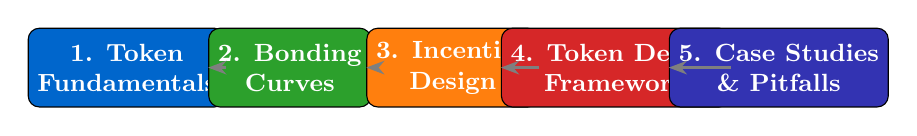
\begin{tikzpicture}[scale=0.9]
  \node[draw,fill=mlblue,text=white,rounded corners=4pt,
        minimum width=2.0cm,minimum height=1.0cm,align=center,font=\small\bfseries]
        (b1) at (0,0) {1. Token\\Fundamentals};
  \node[draw,fill=mlgreen,text=white,rounded corners=4pt,
        minimum width=2.0cm,minimum height=1.0cm,align=center,font=\small\bfseries]
        (b2) at (2.3,0) {2. Bonding\\Curves};
  \node[draw,fill=mlorange,text=white,rounded corners=4pt,
        minimum width=2.0cm,minimum height=1.0cm,align=center,font=\small\bfseries]
        (b3) at (4.6,0) {3. Incentive\\Design};
  \node[draw,fill=mlred,text=white,rounded corners=4pt,
        minimum width=2.0cm,minimum height=1.0cm,align=center,font=\small\bfseries]
        (b4) at (6.9,0) {4. Token Design\\Framework};
  \node[draw,fill=mlpurple,text=white,rounded corners=4pt,
        minimum width=2.0cm,minimum height=1.0cm,align=center,font=\small\bfseries]
        (b5) at (9.2,0) {5. Case Studies\\\& Pitfalls};
  \draw[-{Stealth},thick,mlgray] (b1.east) -- (b2.west);
  \draw[-{Stealth},thick,mlgray] (b2.east) -- (b3.west);
  \draw[-{Stealth},thick,mlgray] (b3.east) -- (b4.west);
  \draw[-{Stealth},thick,mlgray] (b4.east) -- (b5.west);
\end{tikzpicture}
\vspace{3mm}

\column{0.45\textwidth}
\begin{block}{Learning Objectives}
\footnotesize
\begin{itemize}
  \item Classify tokens by function (utility, governance, security)
  \item Analyse supply models and their economic implications
  \item Derive bonding-curve pricing mathematics
  \item Apply game theory to incentive alignment
  \item Design a token economy from first principles
\end{itemize}
\end{block}
\vspace{1mm}
\begin{block}{Prerequisites}
\footnotesize
\begin{itemize}
  \item Lessons 1--5: Blockchain fundamentals, smart contracts, DeFi
  \item Basic familiarity with Ethereum and ERC-20 tokens
\end{itemize}
\end{block}
\end{columns}
\bottomnote{Duration: 90 minutes | 5 sections | \textasciitilde55 frames | Prerequisite: Lessons 1--5}
\end{frame}

% Frame 3: Table of Contents
\begin{frame}{Table of Contents}
\tableofcontents
\bottomnote{Navigate through 5 sections covering token fundamentals to case studies and pitfalls}
\end{frame}

\begin{frame}{Learning Objectives}
By the end of this lecture, you will be able to:
\begin{enumerate}
\item \textbf{Analyze} token supply models (fixed, inflationary, deflationary) and velocity sinks
\item \textbf{Calculate} bonding curve prices using linear, polynomial, and Bancor formulas
\item \textbf{Apply} mechanism design principles (Nash equilibrium, Schelling points) to token systems
\item \textbf{Design} a token using the 7-step framework (utility, distribution, vesting, launch)
\item \textbf{Evaluate} real-world tokenomics through UNI, MKR/DAI, CRV, and LUNA/UST case studies
\end{enumerate}
\bottomnote{Bloom's taxonomy levels: Remember $\rightarrow$ Understand $\rightarrow$ Apply $\rightarrow$ Analyze $\rightarrow$ Evaluate $\rightarrow$ Create}
\end{frame}

%% ============================================================
%% SECTION 1: TOKEN FUNDAMENTALS & SUPPLY ECONOMICS
%% ============================================================
\section{Token Fundamentals \& Supply Economics}

\begin{frame}{}
\begin{beamercolorbox}[sep=12pt,center,rounded=true,shadow=true]{palette quaternary}
{\Large\bfseries Section 1: Token Fundamentals \& Supply Economics}\\[6pt]
{\normalsize Token types, supply mechanics, and valuation fundamentals}
\end{beamercolorbox}
\end{frame}

% Frame 4: What Is a Token?
\begin{frame}{What Is a Token?}
\begin{columns}[T]
\column{0.5\textwidth}
\begin{block}{Definition}
\footnotesize
A \textbf{token} is a digital asset on a blockchain representing a unit of value, utility, or ownership right within a specific ecosystem.
\end{block}
\vspace{2mm}
\begin{block}{Token vs.\ Coin}
\footnotesize
\begin{tabular}{lcc}
\toprule
\textbf{Property} & \textbf{Coin} & \textbf{Token} \\
\midrule
Own blockchain & \textcolor{mlgreen}{\checkmark} & \textcolor{mlred}{$\times$} \\
Native asset & \textcolor{mlgreen}{\checkmark} & \textcolor{mlred}{$\times$} \\
Built on another chain & \textcolor{mlred}{$\times$} & \textcolor{mlgreen}{\checkmark} \\
Smart contract based & \textcolor{mlred}{$\times$} & \textcolor{mlgreen}{\checkmark} \\
\bottomrule
\end{tabular}
\end{block}

\column{0.5\textwidth}
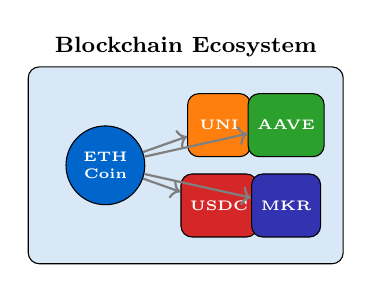
\begin{tikzpicture}[scale=0.85]
  \node[draw,fill=mlblue!15,rounded corners,minimum width=4cm,minimum height=2.5cm] (outer) at (0,0) {};
  \node[above] at (outer.north) {\footnotesize\textbf{Blockchain Ecosystem}};
  \node[draw,fill=mlblue,text=white,circle,minimum size=1cm,font=\tiny\bfseries,align=center] (coin) at (-1.2,0) {ETH\\Coin};
  \node[draw,fill=mlorange,text=white,rounded corners,minimum size=0.8cm,font=\tiny\bfseries] (t1) at (0.5,0.6) {UNI};
  \node[draw,fill=mlgreen,text=white,rounded corners,minimum size=0.8cm,font=\tiny\bfseries] (t2) at (1.5,0.6) {AAVE};
  \node[draw,fill=mlred,text=white,rounded corners,minimum size=0.8cm,font=\tiny\bfseries] (t3) at (0.5,-0.6) {USDC};
  \node[draw,fill=mlpurple,text=white,rounded corners,minimum size=0.8cm,font=\tiny\bfseries] (t4) at (1.5,-0.6) {MKR};
  \draw[->,mlgray,thick] (coin) -- (t1);
  \draw[->,mlgray,thick] (coin) -- (t2);
  \draw[->,mlgray,thick] (coin) -- (t3);
  \draw[->,mlgray,thick] (coin) -- (t4);
\end{tikzpicture}
\end{columns}
\bottomnote{Tokens are programmable assets -- coins are native currencies of their own blockchain}
\end{frame}

% Frame 5: Token Taxonomy
\begin{frame}{Token Taxonomy}
\adjustbox{max width=\textwidth}{%
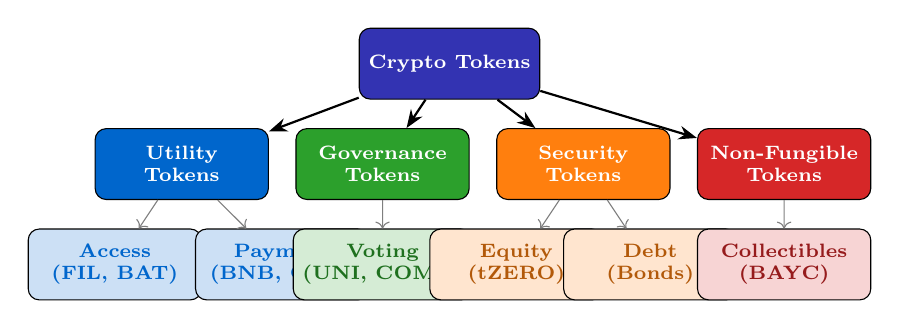
\begin{tikzpicture}[scale=0.85,
  box/.style={draw,rounded corners=4pt,minimum width=2.2cm,minimum height=0.9cm,align=center,font=\scriptsize\bfseries}]
  \node[box,fill=mlpurple,text=white] (root) at (5,3.5) {Crypto Tokens};
  \node[box,fill=mlblue,text=white] (util) at (1,2) {Utility\\Tokens};
  \node[box,fill=mlgreen,text=white] (gov) at (4,2) {Governance\\Tokens};
  \node[box,fill=mlorange,text=white] (sec) at (7,2) {Security\\Tokens};
  \node[box,fill=mlred,text=white] (nft) at (10,2) {Non-Fungible\\Tokens};
  \node[box,fill=mlblue!20,text=mlblue] (u1) at (0,0.5) {Access\\(FIL, BAT)};
  \node[box,fill=mlblue!20,text=mlblue] (u2) at (2.5,0.5) {Payment\\(BNB, CRO)};
  \node[box,fill=mlgreen!20,text=mlgreen!70!black] (g1) at (4,0.5) {Voting\\(UNI, COMP)};
  \node[box,fill=mlorange!20,text=mlorange!70!black] (s1) at (6,0.5) {Equity\\(tZERO)};
  \node[box,fill=mlorange!20,text=mlorange!70!black] (s2) at (8,0.5) {Debt\\(Bonds)};
  \node[box,fill=mlred!20,text=mlred!70!black] (n1) at (10,0.5) {Collectibles\\(BAYC)};
  \draw[-{Stealth},thick] (root) -- (util);
  \draw[-{Stealth},thick] (root) -- (gov);
  \draw[-{Stealth},thick] (root) -- (sec);
  \draw[-{Stealth},thick] (root) -- (nft);
  \draw[->,mlgray] (util) -- (u1);
  \draw[->,mlgray] (util) -- (u2);
  \draw[->,mlgray] (gov) -- (g1);
  \draw[->,mlgray] (sec) -- (s1);
  \draw[->,mlgray] (sec) -- (s2);
  \draw[->,mlgray] (nft) -- (n1);
\end{tikzpicture}
}%
\bottomnote{The SEC's Howey Test determines whether a token qualifies as a security -- implications for compliance}
\end{frame}

% Frame 6: Supply Models Overview
\begin{frame}{Token Supply Models}
\begin{columns}[T]
\column{0.33\textwidth}
\begin{block}{\centering Fixed Supply}
\footnotesize
\begin{itemize}
  \item Hard cap on total tokens
  \item Deflationary pressure
  \item Example: BTC (21M cap)
\end{itemize}
\end{block}
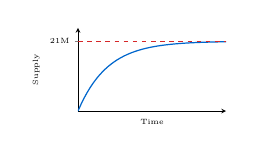
\begin{tikzpicture}[scale=0.55]
\begin{axis}[xlabel={\tiny Time},ylabel={\tiny Supply},width=5cm,height=3.5cm,
  axis lines=left,ymin=0,ymax=25,xmin=0,xmax=10,
  xtick=\empty,ytick={21},yticklabels={\tiny 21M}]
\addplot[mlblue,thick,domain=0:10,samples=50] {21*(1-e^(-0.5*x))};
\draw[dashed,mlred] (axis cs:0,21) -- (axis cs:10,21);
\end{axis}
\end{tikzpicture}

\column{0.33\textwidth}
\begin{block}{\centering Inflationary}
\footnotesize
\begin{itemize}
  \item Continuous new token minting
  \item Funds staking rewards
  \item Example: DOT (\textasciitilde10\%/yr)
\end{itemize}
\end{block}
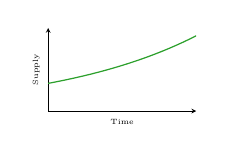
\begin{tikzpicture}[scale=0.55]
\begin{axis}[xlabel={\tiny Time},ylabel={\tiny Supply},width=5cm,height=3.5cm,
  axis lines=left,ymin=0,ymax=30,xmin=0,xmax=10,
  xtick=\empty,ytick=\empty]
\addplot[mlgreen,thick,domain=0:10,samples=50] {10*e^(0.1*x)};
\end{axis}
\end{tikzpicture}

\column{0.33\textwidth}
\begin{block}{\centering Deflationary}
\footnotesize
\begin{itemize}
  \item Burn mechanisms reduce supply
  \item EIP-1559 base fee burn
  \item Example: ETH (post-Merge)
\end{itemize}
\end{block}
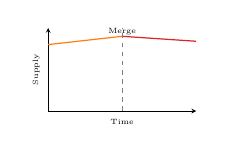
\begin{tikzpicture}[scale=0.55]
\begin{axis}[xlabel={\tiny Time},ylabel={\tiny Supply},width=5cm,height=3.5cm,
  axis lines=left,ymin=0,ymax=25,xmin=0,xmax=10,
  xtick=\empty,ytick=\empty]
\addplot[mlorange,thick,domain=0:5,samples=25] {20+x*0.5};
\addplot[mlred,thick,domain=5:10,samples=25] {22.5-0.3*(x-5)};
\node[font=\tiny] at (axis cs:5,24) {Merge};
\draw[dashed,mlgray] (axis cs:5,0) -- (axis cs:5,25);
\end{axis}
\end{tikzpicture}
\end{columns}
\bottomnote{Supply model is the single most important tokenomic decision -- it defines long-term value dynamics}
\end{frame}

% Frame 7: Inflation & Deflation Mechanics
\begin{frame}{Inflation \& Deflation Mechanics}
\begin{columns}[T]
\column{0.5\textwidth}
\begin{block}{Inflationary Mechanisms (Faucets)}
\footnotesize
\begin{itemize}
  \item \textbf{Block rewards:} New tokens per block (BTC, ETH pre-Merge)
  \item \textbf{Staking rewards:} Minted to incentivise validators
  \item \textbf{Liquidity mining:} Rewards for LP providers
  \item \textbf{Airdrops:} Free distribution to grow user base
\end{itemize}
\end{block}
\vspace{1mm}
\begin{alertblock}{\footnotesize Key Metric}
\footnotesize
\textbf{Real yield} = Staking APY $-$ Inflation rate\\
If inflation $>$ yield, holders lose purchasing power.
\end{alertblock}

\column{0.5\textwidth}
\begin{block}{Deflationary Mechanisms (Sinks)}
\footnotesize
\begin{itemize}
  \item \textbf{Fee burns:} EIP-1559 burns base fees (ETH)
  \item \textbf{Buyback \& burn:} Protocol buys and destroys tokens (BNB)
  \item \textbf{Slashing:} Validators lose staked tokens for misbehaviour
  \item \textbf{Usage burns:} Tokens consumed on use (LUNA pre-crash)
\end{itemize}
\end{block}
\vspace{1mm}
\begin{exampleblock}{\footnotesize Equilibrium}
\footnotesize
\textbf{Net emission} = Minting $-$ Burning\\
ETH targets net emission $\approx 0$ (``ultrasound money'').
\end{exampleblock}
\end{columns}
\bottomnote{Sustainable tokenomics balances faucets (emission) and sinks (burns) for long-term stability}
\end{frame}

% Frame 8: Market Cap & Valuation Metrics
\begin{frame}{Market Cap \& Valuation Metrics}
\begin{columns}[T]
\column{0.55\textwidth}
\begin{block}{Key Formulas}
\footnotesize
\begin{align}
\text{Market Cap} &= \text{Price} \times \text{Circulating Supply} \\
\text{FDV} &= \text{Price} \times \text{Max Supply} \\
\text{MC/FDV Ratio} &= \frac{\text{Circulating Supply}}{\text{Max Supply}}
\end{align}
\end{block}
\vspace{2mm}
\begin{block}{Why FDV Matters}
\footnotesize
\begin{itemize}
  \item Low MC/FDV ratio $\Rightarrow$ large future dilution
  \item Token unlocks create selling pressure
  \item Always compare MC \textbf{and} FDV when evaluating projects
\end{itemize}
\end{block}

\column{0.45\textwidth}
\footnotesize
\begin{tabular}{lrrr}
\toprule
\textbf{Token} & \textbf{MC (\$B)} & \textbf{FDV (\$B)} & \textbf{Ratio} \\
\midrule
BTC & 1,200 & 1,200 & 100\% \\
ETH & 400 & 400 & 100\% \\
SOL & 80 & 95 & 84\% \\
ARB & 3.2 & 12.8 & 25\% \\
OP & 2.5 & 11.0 & 23\% \\
\bottomrule
\end{tabular}
\vspace{2mm}
\begin{alertblock}{\footnotesize Warning}
\footnotesize
Low MC/FDV tokens face significant sell pressure as locked tokens unlock over time.
\end{alertblock}
\end{columns}
\bottomnote{FDV reveals the ``true'' valuation -- a \$3B MC with \$13B FDV means 77\% of tokens are still locked}
\end{frame}

% Frame 9: Token Velocity Problem
\begin{frame}{The Token Velocity Problem}
\begin{columns}[T]
\column{0.5\textwidth}
\begin{block}{Equation of Exchange (Fisher)}
\footnotesize
\[
M \times V = P \times Q
\]
\begin{itemize}
  \item $M$ = token supply (monetary base)
  \item $V$ = velocity (turnover rate)
  \item $P$ = price level
  \item $Q$ = quantity of goods/services
\end{itemize}
\end{block}
\vspace{2mm}
\begin{alertblock}{\footnotesize The Problem}
\footnotesize
If $V$ is high (tokens are not held), then $M$ (and thus token price) must be low to satisfy $PQ$.\\[2mm]
\textbf{High velocity = low token value.}
\end{alertblock}

\column{0.5\textwidth}
\begin{block}{Velocity Reduction Strategies}
\footnotesize
\begin{enumerate}
  \item \textbf{Staking:} Lock tokens for rewards (reduces circulating supply)
  \item \textbf{Governance:} Require holding to vote (time-lock)
  \item \textbf{Burn-and-mint:} Users burn tokens for services
  \item \textbf{Work tokens:} Stake to earn right to perform work
  \item \textbf{veCRV model:} Lock for up to 4 years for boosted rewards
\end{enumerate}
\end{block}
\vspace{1mm}
\begin{exampleblock}{\footnotesize Design Principle}
\footnotesize
Good tokenomics creates reasons to \textbf{hold}, not just \textbf{use and sell}.
\end{exampleblock}
\end{columns}
\bottomnote{Kyle Samani (Multicoin Capital): ``Velocity is the killer of token value'' -- design sinks to counteract}
\end{frame}

% Frame 10: Token Sinks & Faucets Framework
\begin{frame}{Token Sinks \& Faucets Framework}
\begin{center}
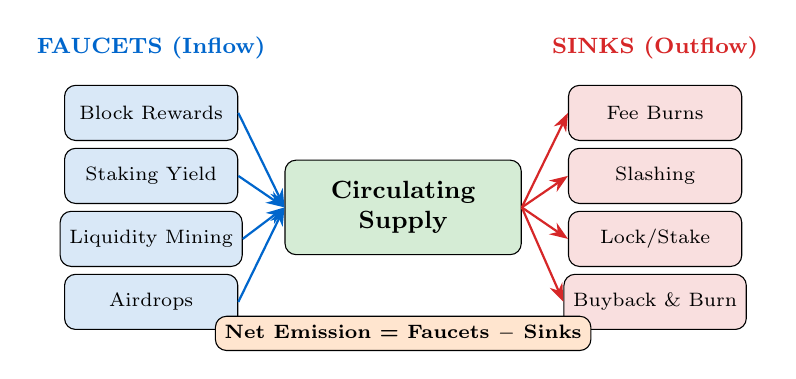
\begin{tikzpicture}[scale=0.8,
  faucet/.style={draw,fill=mlblue!15,rounded corners,minimum width=2.2cm,minimum height=0.7cm,font=\scriptsize,align=center},
  sink/.style={draw,fill=mlred!15,rounded corners,minimum width=2.2cm,minimum height=0.7cm,font=\scriptsize,align=center},
  pool/.style={draw,fill=mlgreen!20,rounded corners,minimum width=3cm,minimum height=1.2cm,font=\small\bfseries,align=center}]
  % Faucets (left)
  \node[faucet] (f1) at (-4,2) {Block Rewards};
  \node[faucet] (f2) at (-4,1) {Staking Yield};
  \node[faucet] (f3) at (-4,0) {Liquidity Mining};
  \node[faucet] (f4) at (-4,-1) {Airdrops};
  \node[above,font=\footnotesize\bfseries,mlblue] at (-4,2.7) {FAUCETS (Inflow)};
  % Pool (center)
  \node[pool] (pool) at (0,0.5) {Circulating\\Supply};
  % Sinks (right)
  \node[sink] (s1) at (4,2) {Fee Burns};
  \node[sink] (s2) at (4,1) {Slashing};
  \node[sink] (s3) at (4,0) {Lock/Stake};
  \node[sink] (s4) at (4,-1) {Buyback \& Burn};
  \node[above,font=\footnotesize\bfseries,mlred] at (4,2.7) {SINKS (Outflow)};
  % Arrows
  \foreach \f in {f1,f2,f3,f4} \draw[-{Stealth},mlblue,thick] (\f.east) -- (pool.west);
  \foreach \s in {s1,s2,s3,s4} \draw[-{Stealth},mlred,thick] (pool.east) -- (\s.west);
  % Equilibrium
  \node[draw,fill=mlorange!20,rounded corners,font=\scriptsize\bfseries] at (0,-1.5) {Net Emission = Faucets $-$ Sinks};
\end{tikzpicture}
\end{center}
\bottomnote{A healthy token economy maintains equilibrium between inflows (faucets) and outflows (sinks)}
\end{frame}

% Frame 11: Circulating Supply Dynamics
\begin{frame}{Circulating Supply Dynamics}
\begin{columns}[T]
\column{0.5\textwidth}
\begin{block}{Supply Categories}
\footnotesize
\begin{itemize}
  \item \textbf{Total Supply:} All tokens that exist
  \item \textbf{Max Supply:} Maximum that can ever exist
  \item \textbf{Circulating Supply:} Tokens freely tradeable
  \item \textbf{Locked Supply:} Vesting, staking, or burned
\end{itemize}
\end{block}
\vspace{2mm}
\footnotesize
\[
\text{Circulating} = \text{Total} - \text{Locked} - \text{Burned}
\]

\column{0.5\textwidth}
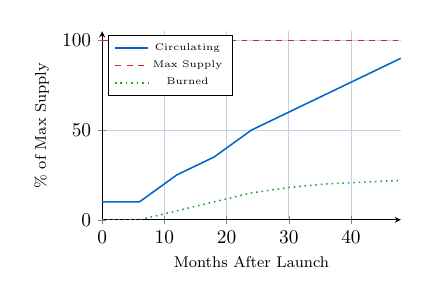
\begin{tikzpicture}[scale=0.7]
\begin{axis}[
  xlabel={\footnotesize Months After Launch},
  ylabel={\footnotesize \% of Max Supply},
  width=7cm,height=5cm,
  axis lines=left,
  ymin=0,ymax=105,xmin=0,xmax=48,
  legend style={font=\tiny,at={(0.02,0.98)},anchor=north west},
  grid=major,grid style={mllavender3}]
\addplot[mlblue,thick,mark=none] coordinates {(0,10)(6,10)(12,25)(18,35)(24,50)(30,60)(36,70)(42,80)(48,90)};
\addplot[mlred,thick,dashed,mark=none] coordinates {(0,100)(6,100)(12,100)(18,100)(24,100)(30,100)(36,100)(42,100)(48,100)};
\addplot[mlgreen,thick,dotted,mark=none] coordinates {(0,0)(6,0)(12,5)(18,10)(24,15)(30,18)(36,20)(42,21)(48,22)};
\legend{Circulating,Max Supply,Burned}
\end{axis}
\end{tikzpicture}
\end{columns}
\bottomnote{Monitor unlock schedules -- large supply releases often correlate with price drops}
\end{frame}

% Frame 12: Halving & Emission Schedules
\begin{frame}{Halving \& Emission Schedules}
\begin{columns}[T]
\column{0.5\textwidth}
\begin{block}{Bitcoin Halving Model}
\footnotesize
Block reward halves every 210,000 blocks (\textasciitilde4 years):
\[
R_n = \frac{50}{2^n} \text{ BTC per block}
\]
\begin{tabular}{ccc}
\toprule
\textbf{Halving} & \textbf{Year} & \textbf{Reward} \\
\midrule
0 & 2009 & 50 BTC \\
1 & 2012 & 25 BTC \\
2 & 2016 & 12.5 BTC \\
3 & 2020 & 6.25 BTC \\
4 & 2024 & 3.125 BTC \\
\bottomrule
\end{tabular}
\end{block}

\column{0.5\textwidth}
\begin{block}{Alternative Emission Models}
\footnotesize
\begin{itemize}
  \item \textbf{Linear decay:} Reward decreases by fixed amount each epoch
  \item \textbf{Tail emission:} Minimum reward forever (Monero: 0.6 XMR/block)
  \item \textbf{Demand-based:} Emission adjusts to network usage (Algorand)
  \item \textbf{Epoch-based:} Discrete reduction at milestones (Solana: $-$15\%/yr)
\end{itemize}
\end{block}
\vspace{1mm}
\begin{exampleblock}{\footnotesize Design Trade-off}
\footnotesize
Aggressive emission $\Rightarrow$ fast bootstrap but dilution\\
Conservative emission $\Rightarrow$ slow growth but value preservation
\end{exampleblock}
\end{columns}
\bottomnote{Stock-to-flow ratio increases with each halving -- scarcity narrative drives price cycles}
\end{frame}

% Frame 13: Real Yield vs. Inflationary Yield
\begin{frame}{Real Yield vs.\ Inflationary Yield}
\begin{columns}[T]
\column{0.5\textwidth}
\begin{block}{Two Sources of DeFi Yield}
\footnotesize
\begin{itemize}
  \item \textbf{Real Yield:} Revenue generated by actual protocol activity (trading fees, interest, liquidation penalties) distributed to token holders.
  \item \textbf{Inflationary Yield:} New tokens minted and distributed as rewards -- effectively diluting existing holders to subsidise new users.
\end{itemize}
\end{block}
\vspace{1mm}
\footnotesize
\[
\text{Real Yield} = \frac{\text{Protocol Revenue to Holders}}{\text{Token Market Cap}} \times 100\%
\]
\[
\text{Effective APY} = \text{Nominal APY} - \text{Inflation Rate}
\]
\vspace{1mm}
\begin{alertblock}{\footnotesize The Sustainability Test}
\footnotesize
If a protocol's yield disappears when token emissions stop, it was \textbf{never real yield} -- it was a temporary subsidy funded by dilution.
\end{alertblock}

\column{0.5\textwidth}
\begin{block}{Comparison}
\footnotesize
\renewcommand{\arraystretch}{1.1}
\begin{tabular}{lcc}
\toprule
\textbf{Dimension} & \textbf{Real Yield} & \textbf{Inflationary} \\
\midrule
Source & Protocol fees & Token emission \\
Sustainable? & Yes & No \\
Dilutive? & No & Yes \\
Typical APY & 3--15\% & 50--1,000\%+ \\
Example & GMX, MKR & Early SUSHI \\
Value signal & Revenue $>$ 0 & Emission $>$ 0 \\
\bottomrule
\end{tabular}
\end{block}
\vspace{2mm}
\begin{exampleblock}{\footnotesize Real Yield Protocols}
\footnotesize
\begin{itemize}
  \item \textbf{GMX:} 30\% of trading fees $\rightarrow$ GMX stakers in ETH/AVAX
  \item \textbf{MakerDAO:} Stability fees buy and burn MKR
  \item \textbf{Lido:} 5\% of staking rewards to LDO treasury
\end{itemize}
\end{exampleblock}
\end{columns}
\bottomnote{DeFi Llama tracks ``Real Yield'' separately from inflationary APY -- always check the source of returns}
\end{frame}

% Frame 14: Section 1 Summary
\begin{frame}{Section 1 Summary: Token Fundamentals}
\begin{columns}[T]
\column{0.5\textwidth}
\begin{block}{Key Concepts}
\footnotesize
\begin{enumerate}
  \item Tokens are programmable assets on existing blockchains
  \item Four main types: utility, governance, security, NFT
  \item Supply model (fixed/inflationary/deflationary) is the core design choice
  \item Market Cap vs.\ FDV reveals dilution risk
  \item Token velocity inversely affects token value
\end{enumerate}
\end{block}

\column{0.5\textwidth}
\begin{block}{Design Checklist}
\footnotesize
\begin{itemize}
  \item[\checkmark] What type of token? (utility, governance, hybrid)
  \item[\checkmark] Fixed or variable supply?
  \item[\checkmark] What are the faucets? (how tokens enter circulation)
  \item[\checkmark] What are the sinks? (how tokens leave circulation)
  \item[\checkmark] What incentivises holding vs.\ selling?
\end{itemize}
\end{block}
\vspace{2mm}
\begin{exampleblock}{\footnotesize Next Section}
\footnotesize
$\Rightarrow$ \textbf{Bonding Curves \& Pricing Mechanisms:} Mathematical foundations for automated token pricing.
\end{exampleblock}
\end{columns}
\bottomnote{Tokenomics is the ``constitution'' of a token economy -- get fundamentals right before mechanism design}
\end{frame}

%% ============================================================
%% SECTION 2: BONDING CURVES & PRICING MECHANISMS
%% ============================================================
\section{Bonding Curves \& Pricing Mechanisms}

\begin{frame}{}
\begin{beamercolorbox}[sep=12pt,center,rounded=true,shadow=true]{palette quaternary}
{\Large\bfseries Section 2: Bonding Curves \& Pricing Mechanisms}\\[6pt]
{\normalsize Automated pricing, bonding curve mathematics, and AMM design}
\end{beamercolorbox}
\end{frame}

% Frame 14: What Is a Bonding Curve?
\begin{frame}{What Is a Bonding Curve?}
\begin{columns}[T]
\column{0.5\textwidth}
\begin{block}{Definition}
\footnotesize
A \textbf{bonding curve} is a mathematical function that defines the relationship between a token's price and its supply. Tokens are minted on purchase and burned on sale via a smart contract.
\end{block}
\vspace{2mm}
\begin{block}{Properties}
\footnotesize
\begin{itemize}
  \item \textbf{Deterministic:} Price is a function of supply
  \item \textbf{Continuous:} Always liquid, no order book needed
  \item \textbf{Autonomous:} No market maker required
  \item \textbf{Transparent:} Price curve is public and immutable
\end{itemize}
\end{block}

\column{0.5\textwidth}
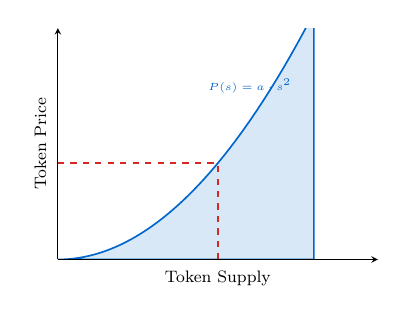
\begin{tikzpicture}[scale=0.75]
\begin{axis}[
  xlabel={\footnotesize Token Supply},
  ylabel={\footnotesize Token Price},
  width=7cm,height=5.5cm,
  axis lines=left,
  ymin=0,ymax=12,xmin=0,xmax=10,
  xtick=\empty,ytick=\empty,
  area style]
\addplot[mlblue,thick,domain=0:8,samples=50,fill=mlblue!15] {0.2*x^2} \closedcycle;
\node[font=\tiny,mlblue] at (axis cs:6,9) {$P(s) = a \cdot s^2$};
\draw[dashed,mlred,thick] (axis cs:5,0) -- (axis cs:5,5);
\draw[dashed,mlred,thick] (axis cs:0,5) -- (axis cs:5,5);
\node[font=\tiny] at (axis cs:5,-0.8) {Current Supply};
\node[font=\tiny,rotate=90] at (axis cs:-0.8,5) {Current Price};
\end{axis}
\end{tikzpicture}
\end{columns}
\bottomnote{Bonding curves enable ``automatic market making'' without counterparties -- pioneered by Bancor in 2017}
\end{frame}

% Frame 15: Linear & Polynomial Curves
\begin{frame}{Linear \& Polynomial Bonding Curves}
\begin{columns}[T]
\column{0.5\textwidth}
\begin{block}{Linear Curve}
\footnotesize
\[
P(s) = m \cdot s + b
\]
\begin{itemize}
  \item Price increases linearly with supply
  \item Constant price sensitivity
  \item Simple but may grow too fast
\end{itemize}
\end{block}
\vspace{1mm}
\begin{block}{Polynomial Curve}
\footnotesize
\[
P(s) = a \cdot s^n
\]
\begin{itemize}
  \item $n < 1$: Sublinear (early buyers benefit less)
  \item $n = 1$: Linear
  \item $n > 1$: Superlinear (early buyers benefit more)
\end{itemize}
\end{block}

\column{0.5\textwidth}
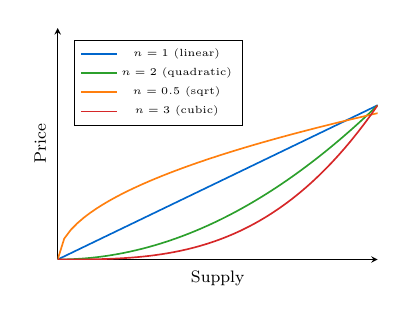
\begin{tikzpicture}[scale=0.75]
\begin{axis}[
  xlabel={\footnotesize Supply},
  ylabel={\footnotesize Price},
  width=7cm,height=5.5cm,
  axis lines=left,
  ymin=0,ymax=15,xmin=0,xmax=10,
  xtick=\empty,ytick=\empty,
  legend style={font=\tiny,at={(0.05,0.95)},anchor=north west}]
\addplot[mlblue,thick,domain=0:10,samples=50] {x};
\addplot[mlgreen,thick,domain=0:10,samples=50] {0.1*x^2};
\addplot[mlorange,thick,domain=0:10,samples=50] {3*x^0.5};
\addplot[mlred,thick,domain=0:10,samples=50] {0.01*x^3};
\legend{$n=1$ (linear),$n=2$ (quadratic),$n=0.5$ (sqrt),$n=3$ (cubic)}
\end{axis}
\end{tikzpicture}
\end{columns}
\bottomnote{Higher exponent $n$ rewards early adopters more aggressively -- choose $n$ based on incentive goals}
\end{frame}

% Frame 16: Bancor Formula
\begin{frame}{The Bancor Formula}
\begin{columns}[T]
\column{0.55\textwidth}
\begin{block}{Continuous Token Model}
\footnotesize
The Bancor protocol introduced the \textbf{Connector Weight} (CW), also called Reserve Ratio:
\[
P = \frac{\text{Reserve Balance}}{\text{Token Supply} \times CW}
\]
\end{block}
\vspace{1mm}
\begin{block}{Purchase Price Calculation}
\footnotesize
Tokens received for depositing $d$ into reserve:
\[
T = S_0 \left[\left(1 + \frac{d}{R_0}\right)^{CW} - 1\right]
\]
where $S_0$ = current supply, $R_0$ = current reserve.
\end{block}
\vspace{1mm}
\begin{exampleblock}{\footnotesize CW Interpretation}
\footnotesize
\begin{itemize}
  \item $CW = 1$: Constant price (stablecoin)
  \item $CW = 0.5$: Linear price increase
  \item $CW < 0.5$: Superlinear (steep curve)
\end{itemize}
\end{exampleblock}

\column{0.45\textwidth}
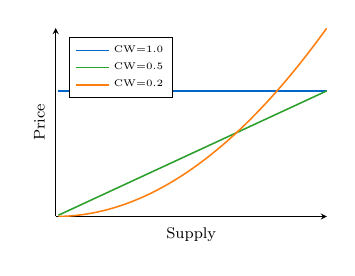
\begin{tikzpicture}[scale=0.7]
\begin{axis}[
  xlabel={\footnotesize Supply},
  ylabel={\footnotesize Price},
  width=6.5cm,height=5cm,
  axis lines=left,
  ymin=0,ymax=15,xmin=0,xmax=10,
  xtick=\empty,ytick=\empty,
  legend style={font=\tiny,at={(0.05,0.95)},anchor=north west}]
\addplot[mlblue,thick,domain=0.1:10,samples=50] {10};
\addplot[mlgreen,thick,domain=0.1:10,samples=50] {x};
\addplot[mlorange,thick,domain=0.1:10,samples=50] {0.15*x^2};
\legend{CW=1.0,CW=0.5,CW=0.2}
\end{axis}
\end{tikzpicture}
\vspace{2mm}
\begin{alertblock}{\footnotesize Slippage}
\footnotesize
Large purchases move along the curve, paying progressively higher prices. This is inherent slippage.
\end{alertblock}
\end{columns}
\bottomnote{Bancor's innovation: algorithmic liquidity without counterparties -- foundation of modern AMMs}
\end{frame}

% Frame 17: Augmented Bonding Curves
\begin{frame}{Augmented Bonding Curves (ABC)}
\begin{columns}[T]
\column{0.55\textwidth}
\begin{block}{Concept (Commons Stack)}
\footnotesize
Augmented bonding curves add a \textbf{funding pool} alongside the reserve pool:
\begin{itemize}
  \item A percentage of each purchase goes to a \textbf{commons fund}
  \item Fund is governed by token holders
  \item Creates sustainable funding for public goods
\end{itemize}
\end{block}
\vspace{2mm}
\begin{block}{Split Mechanism}
\footnotesize
On each buy of amount $d$:
\begin{itemize}
  \item $(1 - \theta) \cdot d$ $\rightarrow$ Reserve (backs token value)
  \item $\theta \cdot d$ $\rightarrow$ Commons Fund (project treasury)
\end{itemize}
Typical $\theta = 0.1$ to $0.3$ (10--30\% to commons).
\end{block}

\column{0.45\textwidth}
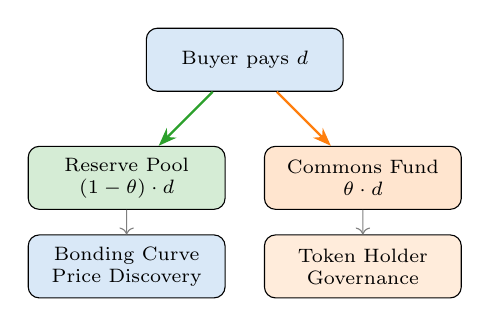
\begin{tikzpicture}[scale=0.75,
  box/.style={draw,rounded corners,minimum width=2.5cm,minimum height=0.8cm,font=\scriptsize,align=center}]
  \node[box,fill=mlblue!15] (buyer) at (0,3) {Buyer pays $d$};
  \node[box,fill=mlgreen!20] (reserve) at (-2,1) {Reserve Pool\\$(1-\theta)\cdot d$};
  \node[box,fill=mlorange!20] (commons) at (2,1) {Commons Fund\\$\theta \cdot d$};
  \node[box,fill=mlblue!15] (curve) at (-2,-0.5) {Bonding Curve\\Price Discovery};
  \node[box,fill=mlorange!15] (gov) at (2,-0.5) {Token Holder\\Governance};
  \draw[-{Stealth},thick,mlgreen] (buyer) -- (reserve);
  \draw[-{Stealth},thick,mlorange] (buyer) -- (commons);
  \draw[->,mlgray] (reserve) -- (curve);
  \draw[->,mlgray] (commons) -- (gov);
\end{tikzpicture}
\end{columns}
\bottomnote{ABCs align speculation with public goods funding -- ``skin in the game'' for ecosystem development}
\end{frame}

% Frame 18: Sigmoid & S-Curve Models
\begin{frame}{Sigmoid \& S-Curve Pricing Models}
\begin{columns}[T]
\column{0.5\textwidth}
\begin{block}{Sigmoid Bonding Curve}
\footnotesize
\[
P(s) = \frac{P_{\max}}{1 + e^{-k(s - s_0)}}
\]
\begin{itemize}
  \item Price starts low, grows rapidly, then plateaus
  \item $P_{\max}$: maximum price ceiling
  \item $s_0$: midpoint of growth
  \item $k$: steepness parameter
\end{itemize}
\end{block}
\vspace{2mm}
\begin{exampleblock}{\footnotesize When to Use Sigmoid}
\footnotesize
\begin{itemize}
  \item Early access at low cost
  \item Natural price ceiling prevents bubbles
  \item Ideal for capped ecosystems
\end{itemize}
\end{exampleblock}

\column{0.5\textwidth}
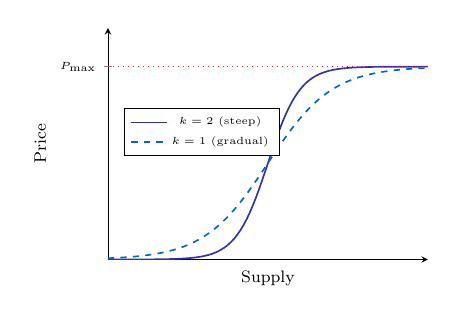
\begin{tikzpicture}[scale=0.75]
\begin{axis}[
  xlabel={\footnotesize Supply},
  ylabel={\footnotesize Price},
  width=7cm,height=5.5cm,
  axis lines=left,
  ymin=0,ymax=12,xmin=0,xmax=10,
  xtick=\empty,ytick={10},yticklabels={\tiny $P_{\max}$},
  legend style={font=\tiny,at={(0.05,0.55)},anchor=west}]
\addplot[mlpurple,thick,domain=0:10,samples=100] {10/(1+exp(-2*(x-5)))};
\addplot[mlblue,thick,dashed,domain=0:10,samples=100] {10/(1+exp(-1*(x-5)))};
\draw[dotted,mlred] (axis cs:0,10) -- (axis cs:10,10);
\legend{$k=2$ (steep),$k=1$ (gradual)}
\end{axis}
\end{tikzpicture}
\end{columns}
\bottomnote{Sigmoid curves are well-suited for tokens that should reach a stable equilibrium price over time}
\end{frame}

% Frame 19: Constant Product AMM (Uniswap)
\begin{frame}{Constant Product AMM (Uniswap Model)}
\begin{columns}[T]
\column{0.5\textwidth}
\begin{block}{Invariant Formula}
\footnotesize
\[
x \cdot y = k
\]
\begin{itemize}
  \item $x$: reserve of token A
  \item $y$: reserve of token B
  \item $k$: constant product invariant
\end{itemize}
\end{block}
\vspace{1mm}
\begin{block}{Marginal Price}
\footnotesize
\[
P = \frac{dy}{dx} = \frac{y}{x}
\]
Trading $\Delta x$ tokens in, receiving:
\[
\Delta y = y - \frac{k}{x + \Delta x} = \frac{y \cdot \Delta x}{x + \Delta x}
\]
\end{block}

\column{0.5\textwidth}
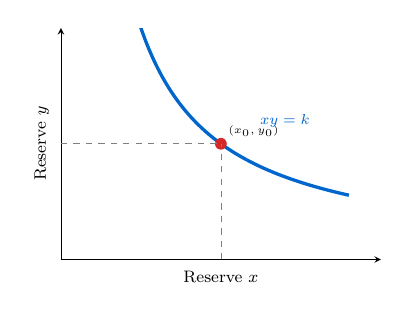
\begin{tikzpicture}[scale=0.75]
\begin{axis}[
  xlabel={\footnotesize Reserve $x$},
  ylabel={\footnotesize Reserve $y$},
  width=7cm,height=5.5cm,
  axis lines=left,
  ymin=0,ymax=20,xmin=0,xmax=20,
  xtick=\empty,ytick=\empty]
\addplot[mlblue,ultra thick,domain=0.8:18,samples=100] {100/x};
\node[circle,fill=mlred,inner sep=2pt] at (axis cs:10,10) {};
\node[font=\tiny,above right] at (axis cs:10,10) {$(x_0,y_0)$};
\draw[dashed,mlgray] (axis cs:10,0) -- (axis cs:10,10);
\draw[dashed,mlgray] (axis cs:0,10) -- (axis cs:10,10);
\node[font=\scriptsize,mlblue] at (axis cs:14,12) {$xy = k$};
\end{axis}
\end{tikzpicture}
\end{columns}
\bottomnote{Uniswap's $xy=k$ is the most widely deployed bonding curve -- over \$1T cumulative volume}
\end{frame}

% Frame 20: Comparing Curve Types
\begin{frame}{Comparing Bonding Curve Types}
\footnotesize
\begin{tabular}{lcccc}
\toprule
\textbf{Property} & \textbf{Linear} & \textbf{Polynomial} & \textbf{Bancor} & \textbf{Sigmoid} \\
\midrule
Formula & $ms + b$ & $as^n$ & $\frac{R}{S \cdot CW}$ & $\frac{P_{\max}}{1+e^{-k(s-s_0)}}$ \\[3mm]
Price ceiling & No & No & No & Yes \\
Early-adopter reward & Moderate & Tunable ($n$) & Tunable (CW) & High \\
Complexity & Low & Low & Medium & Medium \\
Slippage & Predictable & Variable & Variable & Low at extremes \\
Use case & Simple tokens & DAO tokens & DEX reserves & Capped ecosystems \\
\bottomrule
\end{tabular}
\vspace{3mm}
\begin{columns}[T]
\column{0.5\textwidth}
\begin{exampleblock}{\footnotesize Design Guidance}
\footnotesize
Match curve type to your token's purpose:
\begin{itemize}
  \item Fair distribution $\rightarrow$ Linear or sqrt
  \item Reward early adopters $\rightarrow$ Polynomial ($n > 1$)
  \item Sustainable funding $\rightarrow$ Augmented Bancor
\end{itemize}
\end{exampleblock}

\column{0.5\textwidth}
\begin{alertblock}{\footnotesize Common Mistake}
\footnotesize
Using a steep polynomial curve ($n \geq 3$) creates excessive early-adopter advantage, resembling a Ponzi scheme. Regulators scrutinise this.
\end{alertblock}
\end{columns}
\bottomnote{No single curve is ``best'' -- the right choice depends on your distribution goals and regulatory context}
\end{frame}

% Frame 21: Bonding Curve Solidity Implementation
\begin{frame}[fragile]{Bonding Curve: Solidity Implementation}
\begin{lstlisting}
// SPDX-License-Identifier: MIT
pragma solidity ^0.8.20;

contract LinearBondingCurve {
    uint256 public totalSupply;
    uint256 public reserveBalance;
    uint256 public slope = 1e15; // price slope in wei

    mapping(address => uint256) public balances;

    // Price = slope * totalSupply
    function currentPrice() public view returns (uint256) {
        return slope * totalSupply / 1e18;
    }

    // Buy tokens: cost = slope * (s1^2 - s0^2) / 2
    function buy() external payable {
        uint256 s0 = totalSupply;
        // Solve for tokens: area under linear curve
        uint256 tokens = sqrt(2 * msg.value / slope + s0 * s0) - s0;
        totalSupply += tokens;
        reserveBalance += msg.value;
        balances[msg.sender] += tokens;
    }

    function sqrt(uint256 x) internal pure returns (uint256) {
        uint256 z = (x + 1) / 2;
        uint256 y = x;
        while (z < y) { y = z; z = (x / z + z) / 2; }
        return y;
    }
}
\end{lstlisting}
\bottomnote{Production contracts need SafeMath, reentrancy guards, and proper ERC-20 compliance}
\end{frame}

% Frame 22: Liquidity Bootstrapping Pools (LBPs)
\begin{frame}{Liquidity Bootstrapping Pools (LBPs)}
\begin{columns}[T]
\column{0.52\textwidth}
\begin{block}{Mechanism (Balancer LBP)}
\footnotesize
A \textbf{Liquidity Bootstrapping Pool} shifts token weights over time, creating a Dutch-auction-style price discovery:
\begin{itemize}
  \item Start with high project-token weight (e.g., 90/10 TOKEN/USDC)
  \item Gradually shift to balanced ratio (e.g., 50/50) over 24--72 hours
  \item Price starts high and naturally decreases if no one buys
  \item Buyers set their own entry price by choosing when to buy
\end{itemize}
\end{block}
\vspace{1mm}
\begin{block}{Balancer Weighted Pool Price}
\footnotesize
\[
P = \frac{B_{\text{ref}} / w_{\text{ref}}}{B_{\text{token}} / w_{\text{token}}}
\]
As $w_{\text{token}}$ decreases from 0.9 to 0.5 and $w_{\text{ref}}$ increases from 0.1 to 0.5, the denominator grows relative to the numerator, driving price down.
\end{block}

\column{0.48\textwidth}
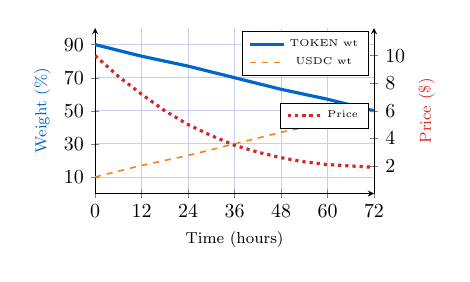
\begin{tikzpicture}[scale=0.72]
\begin{axis}[
  xlabel={\footnotesize Time (hours)},
  width=6.5cm,height=4.5cm,
  axis lines=left,
  axis y line*=left,
  ymin=0,ymax=100,xmin=0,xmax=72,
  ylabel={\footnotesize Weight (\%)},
  ylabel style={mlblue},
  ytick={10,30,50,70,90},
  xtick={0,12,24,36,48,60,72},
  legend style={font=\tiny,at={(0.98,0.98)},anchor=north east},
  grid=major,grid style={mllavender3}]
\addplot[mlblue,ultra thick,mark=none] coordinates {(0,90)(12,83)(24,77)(36,70)(48,63)(60,57)(72,50)};
\addlegendentry{TOKEN wt}
\addplot[mlorange,thick,dashed,mark=none] coordinates {(0,10)(12,17)(24,23)(36,30)(48,37)(60,43)(72,50)};
\addlegendentry{USDC wt}
\end{axis}
\begin{axis}[
  width=6.5cm,height=4.5cm,
  axis lines=right,
  axis x line=none,
  ymin=0,ymax=12,xmin=0,xmax=72,
  ylabel={\footnotesize Price (\$)},
  ylabel style={mlred},
  ytick={2,4,6,8,10},
  legend style={font=\tiny,at={(0.98,0.55)},anchor=north east}]
\addplot[mlred,ultra thick,dotted,mark=none] coordinates {(0,10)(6,8.5)(12,7.2)(18,6)(24,5)(30,4.2)(36,3.5)(42,3.0)(48,2.6)(54,2.3)(60,2.1)(66,2.0)(72,1.9)};
\addlegendentry{Price}
\end{axis}
\end{tikzpicture}
\vspace{1mm}
\begin{exampleblock}{\footnotesize Anti-Bot \& Anti-Whale Properties}
\footnotesize
\begin{itemize}
  \item Bots buying early pay maximum price (self-penalising)
  \item Large buys push price up, rewarding patient small buyers
  \item No front-running advantage -- price declines naturally
\end{itemize}
\end{exampleblock}
\end{columns}
\bottomnote{Balancer LBPs have launched 100+ tokens including Perpetual Protocol, Radicle, and HydraDX}
\end{frame}

% Frame 23: Section 2 Summary
\begin{frame}{Section 2 Summary: Bonding Curves}
\begin{columns}[T]
\column{0.5\textwidth}
\begin{block}{Key Concepts}
\footnotesize
\begin{enumerate}
  \item Bonding curves create deterministic price-supply relationships
  \item Linear, polynomial, Bancor, and sigmoid are the main types
  \item Reserve ratio (CW) controls curve steepness in Bancor model
  \item Augmented curves fund public goods via split mechanism
  \item $xy = k$ (Uniswap) is the most deployed bonding curve
\end{enumerate}
\end{block}

\column{0.5\textwidth}
\begin{block}{Mathematical Toolkit}
\footnotesize
\begin{align}
P_{\text{linear}} &= m \cdot s + b \\
P_{\text{poly}} &= a \cdot s^n \\
P_{\text{bancor}} &= R / (S \cdot CW) \\
P_{\text{sigmoid}} &= P_{\max}/(1 + e^{-k(s-s_0)}) \\
P_{\text{uniswap}} &= y / x
\end{align}
\end{block}
\vspace{2mm}
\begin{exampleblock}{\footnotesize Next Section}
\footnotesize
$\Rightarrow$ \textbf{Incentive Design \& Game Theory:} How to align stakeholder incentives using mechanism design.
\end{exampleblock}
\end{columns}
\bottomnote{Bonding curves are the mathematical backbone of token pricing -- choose wisely for your use case}
\end{frame}

%% ============================================================
%% SECTION 3: INCENTIVE DESIGN & GAME THEORY
%% ============================================================
\section{Incentive Design \& Game Theory}

\begin{frame}{}
\begin{beamercolorbox}[sep=12pt,center,rounded=true,shadow=true]{palette quaternary}
{\Large\bfseries Section 3: Incentive Design \& Game Theory}\\[6pt]
{\normalsize Mechanism design, staking incentives, and Nash equilibria in token systems}
\end{beamercolorbox}
\end{frame}

% Frame 23: Mechanism Design Basics
\begin{frame}{Mechanism Design: The Inverse Game Theory}
\begin{columns}[T]
\column{0.5\textwidth}
\begin{block}{Definition}
\footnotesize
\textbf{Mechanism design} is the engineering side of game theory: instead of analysing existing games, we \textit{design} rules so that rational agents produce desired outcomes.
\end{block}
\vspace{2mm}
\begin{block}{Key Properties}
\footnotesize
\begin{itemize}
  \item \textbf{Incentive compatibility:} Truthful behaviour is optimal
  \item \textbf{Individual rationality:} Participation is voluntary and beneficial
  \item \textbf{Budget balance:} Mechanism doesn't require external funding
\end{itemize}
\end{block}

\column{0.5\textwidth}
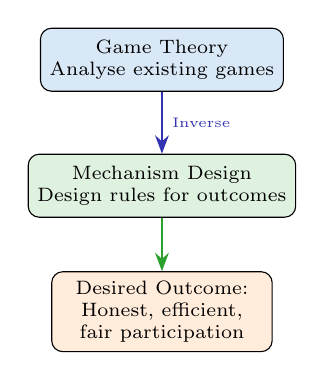
\begin{tikzpicture}[scale=0.8,
  box/.style={draw,rounded corners,minimum width=2.8cm,minimum height=0.8cm,font=\scriptsize,align=center}]
  \node[box,fill=mlblue!15] (gt) at (0,2.5) {Game Theory\\Analyse existing games};
  \node[box,fill=mlgreen!15] (md) at (0,0.5) {Mechanism Design\\Design rules for outcomes};
  \draw[-{Stealth},thick,mlpurple] (gt) -- node[right,font=\tiny] {Inverse} (md);
  \node[box,fill=mlorange!15] (out) at (0,-1.5) {Desired Outcome:\\Honest, efficient,\\fair participation};
  \draw[-{Stealth},thick,mlgreen] (md) -- (out);
\end{tikzpicture}
\end{columns}
\bottomnote{Leonid Hurwicz, Roger Myerson, Eric Maskin won the 2007 Nobel Prize for mechanism design theory}
\end{frame}

% Frame 24: Nash Equilibrium in Token Systems
\begin{frame}{Nash Equilibrium in Token Systems}
\begin{columns}[T]
\column{0.55\textwidth}
\begin{block}{Staking Game: Payoff Matrix}
\footnotesize
Two validators decide whether to \textbf{Stake honestly} or \textbf{Attack}:
\end{block}
\vspace{1mm}
\footnotesize
\begin{tabular}{cc|c|c|}
  & \multicolumn{1}{c}{} & \multicolumn{2}{c}{\textbf{Validator B}} \\
  & & Stake & Attack \\
\cline{3-4}
\multirow{2}{*}{\textbf{Val.~A}} & Stake & \cellcolor{mlgreen!20} 5, 5 & \cellcolor{mlorange!20} 2, 7 \\
\cline{3-4}
  & Attack & \cellcolor{mlorange!20} 7, 2 & \cellcolor{mlred!20} $-$10, $-$10 \\
\cline{3-4}
\end{tabular}
\vspace{2mm}
\begin{alertblock}{\footnotesize Without Slashing}
\footnotesize
(Attack, Attack) is tempting $\rightarrow$ Prisoner's dilemma. Both defect, both lose.
\end{alertblock}

\column{0.45\textwidth}
\begin{block}{With Slashing Penalty}
\footnotesize
Adding slashing ($-20$ for attack detected):
\end{block}
\vspace{1mm}
\footnotesize
\begin{tabular}{c|c|c|}
  & Stake & Attack \\
\hline
Stake & \cellcolor{mlgreen!20} 5, 5 & \cellcolor{mlgreen!20} 5, $-$13 \\
\hline
Attack & \cellcolor{mlgreen!20} $-$13, 5 & \cellcolor{mlred!20} $-$30, $-$30 \\
\hline
\end{tabular}
\vspace{2mm}
\begin{exampleblock}{\footnotesize Nash Equilibrium}
\footnotesize
With slashing, \textbf{(Stake, Stake)} becomes the dominant strategy. Rational validators always stake honestly.
\end{exampleblock}
\end{columns}
\bottomnote{Slashing transforms the game from Prisoner's Dilemma to one where cooperation is the Nash equilibrium}
\end{frame}

% Frame 25: Staking Incentive Design
\begin{frame}{Staking Incentive Design}
\begin{columns}[T]
\column{0.55\textwidth}
\begin{block}{Reward Function}
\footnotesize
Validator reward per epoch:
\[
R_v = R_{\text{base}} \cdot \frac{S_v}{\sum_{i} S_i} \cdot (1 + \beta \cdot \text{uptime}_v)
\]
\begin{itemize}
  \item $S_v$: validator's stake (proportional share)
  \item $R_{\text{base}}$: total rewards per epoch
  \item $\beta$: uptime bonus factor
\end{itemize}
\end{block}
\vspace{1mm}
\begin{block}{Slashing Conditions}
\footnotesize
\begin{itemize}
  \item \textbf{Double signing:} Sign two blocks at same height ($-$5\%)
  \item \textbf{Downtime:} Offline for extended period ($-$0.1\%/epoch)
  \item \textbf{Surround vote:} Contradictory attestations ($-$100\%)
\end{itemize}
\end{block}

\column{0.45\textwidth}
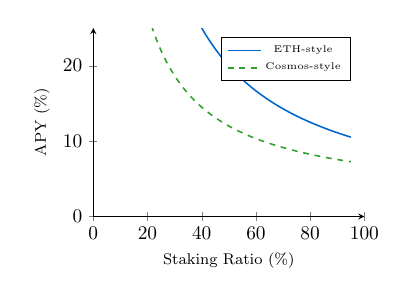
\begin{tikzpicture}[scale=0.7]
\begin{axis}[
  xlabel={\footnotesize Staking Ratio (\%)},
  ylabel={\footnotesize APY (\%)},
  width=6.5cm,height=5cm,
  axis lines=left,
  ymin=0,ymax=25,xmin=0,xmax=100,
  legend style={font=\tiny,at={(0.95,0.95)},anchor=north east}]
\addplot[mlblue,thick,domain=5:95,samples=50] {1000/x};
\addplot[mlgreen,thick,dashed,domain=5:95,samples=50] {500/x + 2};
\legend{ETH-style,Cosmos-style}
\end{axis}
\end{tikzpicture}
\vspace{1mm}
\footnotesize
\textbf{Key insight:} APY decreases as more stake joins $\rightarrow$ self-regulating equilibrium.
\end{columns}
\bottomnote{Ethereum targets 27\% staking ratio -- rewards adjust dynamically to maintain this equilibrium}
\end{frame}

% Frame 26: Tragedy of the Commons in Governance
\begin{frame}{Tragedy of the Commons in Token Governance}
\begin{columns}[T]
\column{0.5\textwidth}
\begin{block}{The Problem}
\footnotesize
\begin{itemize}
  \item Governance is a \textbf{public good}: everyone benefits, few contribute
  \item Rational token holders free-ride: holding is profitable, voting is costly
  \item Result: low participation, plutocratic outcomes
\end{itemize}
\end{block}
\vspace{2mm}
\begin{alertblock}{\footnotesize Real-World Data}
\footnotesize
\begin{tabular}{lr}
\toprule
\textbf{Protocol} & \textbf{Avg.\ Turnout} \\
\midrule
Uniswap & 3--5\% \\
Compound & 5--10\% \\
Aave & 2--4\% \\
MakerDAO & 10--15\% \\
\bottomrule
\end{tabular}
\end{alertblock}

\column{0.5\textwidth}
\begin{block}{Solutions}
\footnotesize
\begin{enumerate}
  \item \textbf{Delegation:} Token holders delegate votes to experts (dPoS-like)
  \item \textbf{Quadratic voting:} Cost = (votes)$^2$, reduces whale dominance
  \item \textbf{Conviction voting:} Voting power grows over time (Gardens)
  \item \textbf{Vote-escrowed:} Lock tokens for boosted governance power (veCRV)
  \item \textbf{Incentivised voting:} Rewards for participation (OP RetroPGF)
\end{enumerate}
\end{block}
\vspace{1mm}
\begin{exampleblock}{\footnotesize Quadratic Voting Cost}
\footnotesize
\[
\text{Cost}(n) = n^2 \text{ tokens for } n \text{ votes}
\]
1 vote = 1 token, 10 votes = 100 tokens.
\end{exampleblock}
\end{columns}
\bottomnote{Low governance turnout is the \#1 challenge in DAO design -- mechanism design must incentivise participation}
\end{frame}

% Frame 27: MEV and Strategic Behaviour
\begin{frame}{MEV and Strategic Behaviour}
\begin{columns}[T]
\column{0.5\textwidth}
\begin{block}{Maximal Extractable Value (MEV)}
\footnotesize
\textbf{MEV} = profit extracted by reordering, inserting, or censoring transactions within a block.
\end{block}
\vspace{1mm}
\begin{block}{MEV Strategies}
\footnotesize
\begin{itemize}
  \item \textbf{Frontrunning:} Insert tx before a known large trade
  \item \textbf{Backrunning:} Insert tx after an oracle update
  \item \textbf{Sandwich attack:} Buy before, sell after a victim's trade
  \item \textbf{Liquidation:} Race to liquidate undercollateralised positions
\end{itemize}
\end{block}

\column{0.5\textwidth}
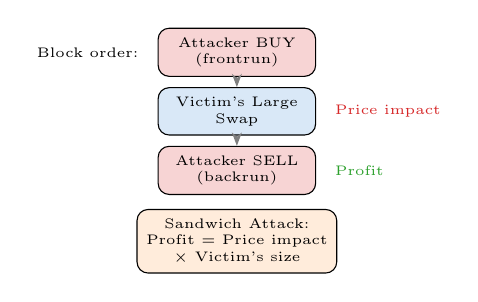
\begin{tikzpicture}[scale=0.75,
  tx/.style={draw,rounded corners,minimum width=2cm,minimum height=0.6cm,font=\tiny,align=center}]
  \node[tx,fill=mlred!20] (front) at (0,2.5) {Attacker BUY\\(frontrun)};
  \node[tx,fill=mlblue!15] (victim) at (0,1.5) {Victim's Large\\Swap};
  \node[tx,fill=mlred!20] (back) at (0,0.5) {Attacker SELL\\(backrun)};
  \draw[-{Stealth},mlgray] (front) -- (victim);
  \draw[-{Stealth},mlgray] (victim) -- (back);
  \node[left,font=\tiny] at (-1.5,2.5) {Block order:};
  \node[right,font=\tiny,mlred] at (1.5,1.5) {Price impact};
  \node[right,font=\tiny,mlgreen] at (1.5,0.5) {Profit};
  \node[draw,fill=mlorange!15,rounded corners,font=\tiny,align=center] at (0,-0.7) {Sandwich Attack:\\Profit = Price impact\\$\times$ Victim's size};
\end{tikzpicture}
\end{columns}
\bottomnote{Flashbots estimates \$600M+ MEV extracted on Ethereum -- mechanism design must account for strategic actors}
\end{frame}

% Frame 28: Schelling Points & Coordination Games
\begin{frame}{Schelling Points \& Coordination Games}
\begin{columns}[T]
\column{0.5\textwidth}
\begin{block}{Schelling Point}
\footnotesize
A \textbf{Schelling point} (focal point) is a solution people converge on without communication, because it seems natural or obvious.
\end{block}
\vspace{2mm}
\begin{block}{Oracle Design Example (Chainlink)}
\footnotesize
\begin{itemize}
  \item $N$ oracle nodes independently report ETH/USD price
  \item Honest reporting is the Schelling point
  \item Outliers are penalised (slashed)
  \item Median value is accepted as ``truth''
\end{itemize}
\end{block}
\vspace{1mm}
\begin{exampleblock}{\footnotesize Reward Function}
\footnotesize
\[
R_i = \begin{cases} R_{\text{base}} & \text{if } |p_i - \tilde{p}| < \epsilon \\ -S_{\text{slash}} & \text{otherwise} \end{cases}
\]
\end{exampleblock}

\column{0.5\textwidth}
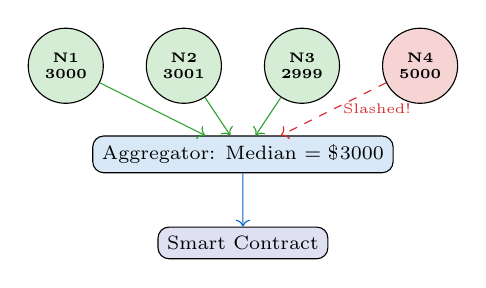
\begin{tikzpicture}[scale=0.75,
  node/.style={draw,circle,minimum size=0.8cm,font=\tiny\bfseries,align=center}]
  \node[node,fill=mlgreen!20] (n1) at (0,3) {N1\\3000};
  \node[node,fill=mlgreen!20] (n2) at (2,3) {N2\\3001};
  \node[node,fill=mlgreen!20] (n3) at (4,3) {N3\\2999};
  \node[node,fill=mlred!20] (n4) at (6,3) {N4\\5000};
  \node[draw,fill=mlblue!15,rounded corners,minimum width=3cm,font=\scriptsize] (agg) at (3,1.5) {Aggregator: Median = \$3000};
  \node[draw,fill=mlpurple!15,rounded corners,minimum width=2cm,font=\scriptsize] (sc) at (3,0) {Smart Contract};
  \draw[->,mlgreen] (n1) -- (agg);
  \draw[->,mlgreen] (n2) -- (agg);
  \draw[->,mlgreen] (n3) -- (agg);
  \draw[->,mlred,dashed] (n4) -- (agg) node[midway,right,font=\tiny,mlred] {Slashed!};
  \draw[->,mlblue] (agg) -- (sc);
\end{tikzpicture}
\end{columns}
\bottomnote{Schelling point mechanisms underpin oracle networks, prediction markets, and dispute resolution systems}
\end{frame}

% Frame 29: Token-Curated Registries
\begin{frame}{Token-Curated Registries (TCRs)}
\begin{columns}[T]
\column{0.5\textwidth}
\begin{block}{Mechanism}
\footnotesize
A \textbf{TCR} is a decentralised list curated by token holders:
\begin{enumerate}
  \item Applicant stakes tokens to apply for listing
  \item Challenge period: anyone can challenge by staking
  \item If challenged $\rightarrow$ token-weighted vote
  \item Winner keeps loser's stake (incentive alignment)
\end{enumerate}
\end{block}
\vspace{2mm}
\begin{block}{Game-Theoretic Incentives}
\footnotesize
\begin{itemize}
  \item \textbf{Applicants:} Only apply if genuinely qualified (risk losing stake)
  \item \textbf{Challengers:} Only challenge bad applications (risk losing stake)
  \item \textbf{Voters:} Vote honestly (earn share of loser's stake)
\end{itemize}
\end{block}

\column{0.5\textwidth}
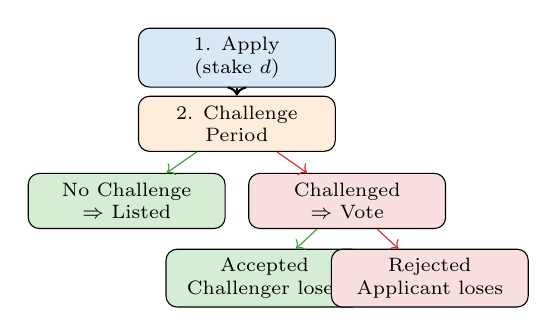
\begin{tikzpicture}[scale=0.7,
  stp/.style={draw,rounded corners,minimum width=2.5cm,minimum height=0.7cm,font=\scriptsize,align=center}]
  \node[stp,fill=mlblue!15] (s1) at (0,4) {1. Apply\\(stake $d$)};
  \node[stp,fill=mlorange!15] (s2) at (0,2.8) {2. Challenge\\Period};
  \node[stp,fill=mlgreen!20] (s3a) at (-2,1.4) {No Challenge\\$\Rightarrow$ Listed};
  \node[stp,fill=mlred!15] (s3b) at (2,1.4) {Challenged\\$\Rightarrow$ Vote};
  \node[stp,fill=mlgreen!20] (s4a) at (0.5,0) {Accepted\\Challenger loses};
  \node[stp,fill=mlred!15] (s4b) at (3.5,0) {Rejected\\Applicant loses};
  \draw[->,thick] (s1) -- (s2);
  \draw[->,mlgreen] (s2) -- (s3a);
  \draw[->,mlred] (s2) -- (s3b);
  \draw[->,mlgreen] (s3b) -- (s4a);
  \draw[->,mlred] (s3b) -- (s4b);
\end{tikzpicture}
\end{columns}
\bottomnote{TCRs demonstrate how skin-in-the-game via staking creates self-policing communities}
\end{frame}

% Frame 30: Incentive Failure Modes
\begin{frame}{Incentive Failure Modes}
\begin{columns}[T]
\column{0.5\textwidth}
\begin{block}{Mercenary Capital}
\footnotesize
\begin{itemize}
  \item Liquidity providers chase highest APY
  \item Leave immediately when rewards decrease
  \item Destabilises protocol TVL
  \item Solution: time-locked rewards, veCRV model
\end{itemize}
\end{block}
\vspace{2mm}
\begin{block}{Governance Attacks}
\footnotesize
\begin{itemize}
  \item Flash loan to acquire voting power
  \item Pass malicious proposal in single tx
  \item Example: Beanstalk \$182M governance attack (2022)
  \item Solution: time-locks, vote-escrow, snapshot voting
\end{itemize}
\end{block}

\column{0.5\textwidth}
\begin{block}{Sybil Attacks on Airdrops}
\footnotesize
\begin{itemize}
  \item Create thousands of wallets
  \item Qualify each for airdrop criteria
  \item Dump tokens immediately
  \item Solution: identity verification, retroactive criteria
\end{itemize}
\end{block}
\vspace{2mm}
\begin{alertblock}{\footnotesize Death Spirals}
\footnotesize
Reflexive feedback loops where falling price triggers more selling:
\begin{enumerate}
  \item Price drops $\rightarrow$ collateral under-backed
  \item Liquidations fire $\rightarrow$ more selling pressure
  \item Confidence collapses $\rightarrow$ bank run
  \item Example: UST/LUNA May 2022
\end{enumerate}
\end{alertblock}
\end{columns}
\bottomnote{Every incentive mechanism has attack vectors -- adversarial thinking is essential in tokenomic design}
\end{frame}

% Frame 31: Quadratic Voting & Funding
\begin{frame}{Quadratic Voting \& Quadratic Funding}
\begin{columns}[T]
\column{0.5\textwidth}
\begin{block}{Quadratic Voting (QV)}
\footnotesize
In standard token voting, 1 token = 1 vote $\Rightarrow$ plutocratic.\\[1mm]
\textbf{QV:} Cost to cast $v$ votes = $v^2$ tokens.
\[
\text{Cost}(v) = v^2 \quad \Rightarrow \quad v = \sqrt{\text{tokens spent}}
\]
\begin{itemize}
  \item Buying 1 vote costs 1 token, 2 votes cost 4, 10 votes cost 100
  \item Reduces whale dominance: a whale with 10,000 tokens gets 100 votes, not 10,000
  \item Expresses \emph{preference intensity} -- voters can allocate more to issues they care about
\end{itemize}
\end{block}
\vspace{1mm}
\begin{exampleblock}{\footnotesize QV Comparison}
\footnotesize
\begin{tabular}{lcc}
\toprule
\textbf{Tokens} & \textbf{1-token-1-vote} & \textbf{QV ($\sqrt{}$)} \\
\midrule
1 & 1 & 1 \\
100 & 100 & 10 \\
10,000 & 10,000 & 100 \\
1,000,000 & 1,000,000 & 1,000 \\
\bottomrule
\end{tabular}
\end{exampleblock}

\column{0.5\textwidth}
\begin{block}{Quadratic Funding (Gitcoin Grants)}
\footnotesize
\textbf{Matching formula} from Buterin, Hitzig \& Weyl (2019):
\[
F_i = \left(\sum_{j=1}^{n} \sqrt{c_{ij}}\right)^2
\]
where $c_{ij}$ is contributor $j$'s donation to project $i$.\\[1mm]
\textbf{Key property:} Many small contributions are amplified more than few large ones.
\end{block}
\vspace{1mm}
\footnotesize
\textbf{Example:} Project A gets \$1 from 100 people; Project B gets \$100 from 1 person.
\begin{itemize}
  \item Direct total: both receive \$100
  \item QF matching: $A = (100 \times \sqrt{1})^2 = \$10{,}000$;\\ $B = (1 \times \sqrt{100})^2 = \$100$
  \item Project A receives 100$\times$ more matching -- reflecting broader support
\end{itemize}
\vspace{1mm}
\begin{alertblock}{\footnotesize Challenges}
\footnotesize
\begin{itemize}
  \item Sybil attacks: split one identity into many to game matching
  \item Collusion: coordinated voting rings
  \item Solutions: Gitcoin Passport, MACI (anti-collusion infrastructure)
\end{itemize}
\end{alertblock}
\end{columns}
\bottomnote{Buterin, Hitzig \& Weyl, ``Liberal Radicalism'' (2019) -- QF has distributed \$50M+ via Gitcoin to public goods}
\end{frame}

% Frame 32: Section 3 Summary
\begin{frame}{Section 3 Summary: Incentive Design}
\begin{columns}[T]
\column{0.5\textwidth}
\begin{block}{Key Concepts}
\footnotesize
\begin{enumerate}
  \item Mechanism design engineers rules for desired outcomes
  \item Slashing transforms games to make honesty dominant
  \item Staking APY self-regulates via supply/demand
  \item Quadratic voting reduces plutocratic governance
  \item Schelling points enable decentralised consensus
\end{enumerate}
\end{block}

\column{0.5\textwidth}
\begin{block}{Failure Modes to Watch}
\footnotesize
\begin{itemize}
  \item[\textcolor{mlred}{\textbullet}] Mercenary capital (short-term LPs)
  \item[\textcolor{mlred}{\textbullet}] Flash loan governance attacks
  \item[\textcolor{mlred}{\textbullet}] Sybil attacks on airdrops
  \item[\textcolor{mlred}{\textbullet}] Death spirals (reflexive loops)
  \item[\textcolor{mlred}{\textbullet}] MEV extraction by block producers
\end{itemize}
\end{block}
\vspace{2mm}
\begin{exampleblock}{\footnotesize Next Section}
\footnotesize
$\Rightarrow$ \textbf{Token Design Framework:} Step-by-step methodology for designing your own token economy.
\end{exampleblock}
\end{columns}
\bottomnote{Good mechanism design assumes all participants are rational and self-interested -- then proves honesty is optimal}
\end{frame}

%% ============================================================
%% SECTION 4: TOKEN DESIGN FRAMEWORK
%% ============================================================
\section{Token Design Framework}

\begin{frame}{}
\begin{beamercolorbox}[sep=12pt,center,rounded=true,shadow=true]{palette quaternary}
{\Large\bfseries Section 4: Token Design Framework}\\[6pt]
{\normalsize Systematic methodology for designing sustainable token economies}
\end{beamercolorbox}
\end{frame}

% Frame 32: Token Design Methodology
\begin{frame}{Token Design Methodology: 7-Step Framework}
\begin{center}
\adjustbox{max width=\textwidth}{%
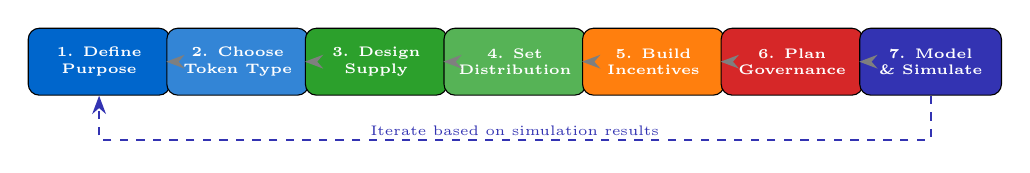
\begin{tikzpicture}[scale=0.8,
  stp/.style={draw,rounded corners=4pt,minimum width=1.8cm,minimum height=0.85cm,align=center,font=\tiny\bfseries}]
  \node[stp,fill=mlblue,text=white] (s1) at (0,0) {1. Define\\Purpose};
  \node[stp,fill=mlblue!80!white,text=white] (s2) at (2.2,0) {2. Choose\\Token Type};
  \node[stp,fill=mlgreen,text=white] (s3) at (4.4,0) {3. Design\\Supply};
  \node[stp,fill=mlgreen!80!white,text=white] (s4) at (6.6,0) {4. Set\\Distribution};
  \node[stp,fill=mlorange,text=white] (s5) at (8.8,0) {5. Build\\Incentives};
  \node[stp,fill=mlred,text=white] (s6) at (11,0) {6. Plan\\Governance};
  \node[stp,fill=mlpurple,text=white] (s7) at (13.2,0) {7. Model\\\& Simulate};
  \draw[-{Stealth},thick,mlgray] (s1) -- (s2);
  \draw[-{Stealth},thick,mlgray] (s2) -- (s3);
  \draw[-{Stealth},thick,mlgray] (s3) -- (s4);
  \draw[-{Stealth},thick,mlgray] (s4) -- (s5);
  \draw[-{Stealth},thick,mlgray] (s5) -- (s6);
  \draw[-{Stealth},thick,mlgray] (s6) -- (s7);
  % Feedback loop
  \draw[-{Stealth},thick,mlpurple,dashed] (s7.south) -- ++(0,-0.7) -| (s1.south);
  \node[font=\tiny,mlpurple] at (6.6,-1.1) {Iterate based on simulation results};
\end{tikzpicture}
}%
\end{center}
\vspace{2mm}
\footnotesize
\begin{columns}[T]
\column{0.5\textwidth}
\begin{itemize}
  \item[\textbf{1.}] What problem does the token solve?
  \item[\textbf{2.}] Utility, governance, or hybrid?
  \item[\textbf{3.}] Fixed, inflationary, or deflationary supply?
  \item[\textbf{4.}] Fair launch, ICO, airdrop, or mining?
\end{itemize}
\column{0.5\textwidth}
\begin{itemize}
  \item[\textbf{5.}] What rewards holding? What penalises misbehaviour?
  \item[\textbf{6.}] Who decides what? How do votes work?
  \item[\textbf{7.}] Agent-based simulation before launch
\end{itemize}
\end{columns}
\bottomnote{Token design is iterative -- simulate extensively before deployment because smart contracts are immutable}
\end{frame}

% Frame 33: Value Capture Mechanisms
\begin{frame}{Value Capture Mechanisms}
\begin{columns}[T]
\column{0.5\textwidth}
\begin{block}{How Tokens Capture Value}
\footnotesize
\begin{enumerate}
  \item \textbf{Fee capture:} Protocol fees flow to token holders (Sushi, Curve)
  \item \textbf{Buyback \& burn:} Revenue buys and destroys tokens (BNB)
  \item \textbf{Work token:} Must stake to earn right to perform work (LINK, GRT)
  \item \textbf{Collateral:} Token used as collateral in the system (MKR, AAVE)
  \item \textbf{Access:} Token required to use platform features (FIL, AR)
\end{enumerate}
\end{block}

\column{0.5\textwidth}
\footnotesize
\begin{tabular}{lll}
\toprule
\textbf{Mechanism} & \textbf{Example} & \textbf{Strength} \\
\midrule
Fee sharing & CRV & Direct yield \\
Buyback/burn & BNB & Deflationary \\
Work token & LINK & Demand-driven \\
Collateral & MKR & Systemic need \\
Access gate & FIL & Usage-driven \\
\bottomrule
\end{tabular}
\vspace{3mm}
\begin{alertblock}{\footnotesize The ``Governance Only'' Trap}
\footnotesize
Tokens with \textit{only} governance rights struggle to capture value. Governance alone is not enough demand driver.
\end{alertblock}
\end{columns}
\bottomnote{Strong value capture = strong reason to buy \& hold -- without it, tokens trend toward zero}
\end{frame}

% Frame 34: Distribution Strategies
\begin{frame}{Token Distribution Strategies}
\begin{columns}[T]
\column{0.5\textwidth}
\begin{block}{Distribution Methods}
\footnotesize
\begin{itemize}
  \item \textbf{Fair Launch:} No pre-mine, no VC allocation (BTC, YFI)
  \item \textbf{ICO/IDO:} Public sale at fixed or dynamic price
  \item \textbf{Airdrop:} Free distribution to early users (UNI, ENS)
  \item \textbf{Liquidity Mining:} Earn tokens by providing liquidity
  \item \textbf{VC Rounds:} Seed, Series A, etc.\ with vesting
\end{itemize}
\end{block}

\column{0.5\textwidth}
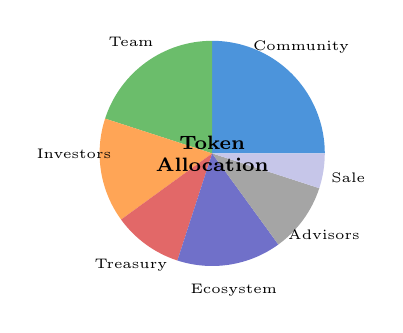
\begin{tikzpicture}[scale=0.65]
  % Pie chart
  \foreach \p/\s/\c/\l [count=\i] in {
    0/25/mlblue/{Community (25\%)},
    25/20/mlgreen/{Team (20\%)},
    45/15/mlorange/{Investors (15\%)},
    60/10/mlred/{Treasury (10\%)},
    70/15/mlpurple/{Ecosystem (15\%)},
    85/10/mlgray/{Advisors (10\%)},
    95/5/mllavender/{Public Sale (5\%)}
  } {
    \pgfmathsetmacro{\sa}{\p*3.6}
    \pgfmathsetmacro{\ea}{(\p+\s)*3.6}
    \fill[\c!70] (0,0) -- (\sa:2.2) arc (\sa:\ea:2.2) -- cycle;
  }
  \node[font=\tiny] at (50:2.7) {Community};
  \node[font=\tiny] at (126:2.7) {Team};
  \node[font=\tiny] at (180:2.7) {Investors};
  \node[font=\tiny] at (234:2.7) {Treasury};
  \node[font=\tiny] at (279:2.7) {Ecosystem};
  \node[font=\tiny] at (324:2.7) {Advisors};
  \node[font=\tiny] at (350:2.7) {Sale};
  \node[font=\scriptsize\bfseries,align=center] at (0,0) {Token\\Allocation};
\end{tikzpicture}
\end{columns}
\bottomnote{Distribution determines who controls the network -- prioritise community allocation for decentralisation}
\end{frame}

% Frame 35: Vesting Schedules & Cliff Periods
\begin{frame}{Vesting Schedules \& Cliff Periods}
\begin{columns}[T]
\column{0.55\textwidth}
\begin{block}{Vesting Terminology}
\footnotesize
\begin{itemize}
  \item \textbf{TGE (Token Generation Event):} Initial token creation
  \item \textbf{Cliff:} Period before any tokens unlock
  \item \textbf{Linear vesting:} Tokens unlock gradually over time
  \item \textbf{TGE unlock:} Percentage available immediately
\end{itemize}
\end{block}
\vspace{2mm}
\footnotesize
\begin{tabular}{lccc}
\toprule
\textbf{Stakeholder} & \textbf{TGE} & \textbf{Cliff} & \textbf{Vesting} \\
\midrule
Team & 0\% & 12 mo & 36 mo linear \\
Investors & 5\% & 6 mo & 24 mo linear \\
Community & 20\% & 0 & 12 mo linear \\
Advisors & 0\% & 6 mo & 24 mo linear \\
\bottomrule
\end{tabular}

\column{0.45\textwidth}
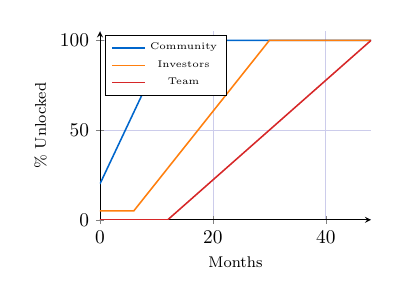
\begin{tikzpicture}[scale=0.7]
\begin{axis}[
  xlabel={\footnotesize Months},
  ylabel={\footnotesize \% Unlocked},
  width=6.5cm,height=5cm,
  axis lines=left,
  ymin=0,ymax=105,xmin=0,xmax=48,
  legend style={font=\tiny,at={(0.02,0.98)},anchor=north west},
  grid=major,grid style={mllavender3}]
% Community: 20% TGE, linear over 12mo
\addplot[mlblue,thick] coordinates {(0,20)(12,100)(48,100)};
% Investors: 5% TGE, 6mo cliff, linear 24mo
\addplot[mlorange,thick] coordinates {(0,5)(6,5)(30,100)(48,100)};
% Team: 0% TGE, 12mo cliff, linear 36mo
\addplot[mlred,thick] coordinates {(0,0)(12,0)(48,100)};
\legend{Community,Investors,Team}
\end{axis}
\end{tikzpicture}
\end{columns}
\bottomnote{Longer team vesting signals commitment -- investors scrutinise vesting schedules for alignment}
\end{frame}

% Frame 36: Vesting Contract in Solidity
\begin{frame}[fragile]{Token Vesting: Solidity Implementation}
\begin{lstlisting}
// SPDX-License-Identifier: MIT
pragma solidity ^0.8.20;

import "@openzeppelin/contracts/token/ERC20/IERC20.sol";

contract TokenVesting {
    IERC20 public token;
    address public beneficiary;
    uint256 public start;
    uint256 public cliff;     // cliff duration in seconds
    uint256 public duration;  // total vesting duration
    uint256 public released;

    constructor(IERC20 _token, address _beneficiary,
                uint256 _cliff, uint256 _duration) {
        token = _token;
        beneficiary = _beneficiary;
        start = block.timestamp;
        cliff = _cliff;
        duration = _duration;
    }

    function releasable() public view returns (uint256) {
        return vestedAmount() - released;
    }

    function vestedAmount() public view returns (uint256) {
        uint256 total = token.balanceOf(address(this)) + released;
        if (block.timestamp < start + cliff) return 0;
        if (block.timestamp >= start + duration) return total;
        return total * (block.timestamp - start) / duration;
    }

    function release() external {
        uint256 amount = releasable();
        require(amount > 0, "Nothing to release");
        released += amount;
        token.transfer(beneficiary, amount);
    }
}
\end{lstlisting}
\bottomnote{OpenZeppelin provides production-ready VestingWallet -- this simplified version illustrates the core logic}
\end{frame}

% Frame 37: Staking Contract in Solidity
\begin{frame}[fragile]{Simple Staking: Solidity Implementation}
\begin{lstlisting}
// SPDX-License-Identifier: MIT
pragma solidity ^0.8.20;

import "@openzeppelin/contracts/token/ERC20/IERC20.sol";

contract SimpleStaking {
    IERC20 public stakingToken;
    uint256 public rewardRate = 100; // tokens per second
    uint256 public lastUpdateTime;
    uint256 public rewardPerTokenStored;
    uint256 public totalStaked;

    mapping(address => uint256) public staked;
    mapping(address => uint256) public rewards;
    mapping(address => uint256) public userRewardPerToken;

    function stake(uint256 amount) external updateReward(msg.sender) {
        totalStaked += amount;
        staked[msg.sender] += amount;
        stakingToken.transferFrom(msg.sender, address(this), amount);
    }

    function withdraw(uint256 amount) external updateReward(msg.sender) {
        totalStaked -= amount;
        staked[msg.sender] -= amount;
        stakingToken.transfer(msg.sender, amount);
    }

    modifier updateReward(address account) {
        rewardPerTokenStored = rewardPerToken();
        lastUpdateTime = block.timestamp;
        rewards[account] = earned(account);
        userRewardPerToken[account] = rewardPerTokenStored;
        _;
    }

    function rewardPerToken() public view returns (uint256) {
        if (totalStaked == 0) return rewardPerTokenStored;
        return rewardPerTokenStored +
            (block.timestamp - lastUpdateTime) * rewardRate * 1e18 / totalStaked;
    }

    function earned(address account) public view returns (uint256) {
        return staked[account] *
            (rewardPerToken() - userRewardPerToken[account]) / 1e18
            + rewards[account];
    }
}
\end{lstlisting}
\bottomnote{Based on Synthetix StakingRewards pattern -- the most widely forked staking contract in DeFi}
\end{frame}

% Frame 38: Token Launch Checklist
\begin{frame}{Token Launch Checklist}
\begin{columns}[T]
\column{0.5\textwidth}
\begin{block}{Pre-Launch}
\footnotesize
\begin{itemize}
  \item[\checkmark] Token purpose and value proposition defined
  \item[\checkmark] Supply model and emission schedule set
  \item[\checkmark] Distribution allocations finalised
  \item[\checkmark] Vesting schedules for all stakeholders
  \item[\checkmark] Smart contracts audited (2+ auditors)
  \item[\checkmark] Legal opinion on token classification
  \item[\checkmark] Agent-based simulation completed
\end{itemize}
\end{block}
\vspace{1mm}
\begin{block}{Launch Day}
\footnotesize
\begin{itemize}
  \item[\checkmark] Liquidity pool seeded
  \item[\checkmark] Token contract verified on Etherscan
  \item[\checkmark] Initial distribution executed
  \item[\checkmark] Governance forum live
\end{itemize}
\end{block}

\column{0.5\textwidth}
\begin{block}{Post-Launch Monitoring}
\footnotesize
\begin{itemize}
  \item[\checkmark] Token velocity tracking
  \item[\checkmark] Holder distribution (Gini coefficient)
  \item[\checkmark] Governance participation rate
  \item[\checkmark] TVL and usage metrics
  \item[\checkmark] Unlock schedule calendar public
\end{itemize}
\end{block}
\vspace{2mm}
\begin{alertblock}{\footnotesize Common Launch Mistakes}
\footnotesize
\begin{enumerate}
  \item Too much TGE unlock (dumping)
  \item No liquidity depth (volatile price)
  \item Unclear value capture mechanism
  \item Team allocation too high ($>$25\%)
\end{enumerate}
\end{alertblock}
\end{columns}
\bottomnote{A token launch is like an IPO -- meticulous preparation and transparent communication are essential}
\end{frame}

% Frame 39: Token Utility Matrix
\begin{frame}{Token Utility Matrix}
\begin{center}
\adjustbox{max width=\textwidth}{%
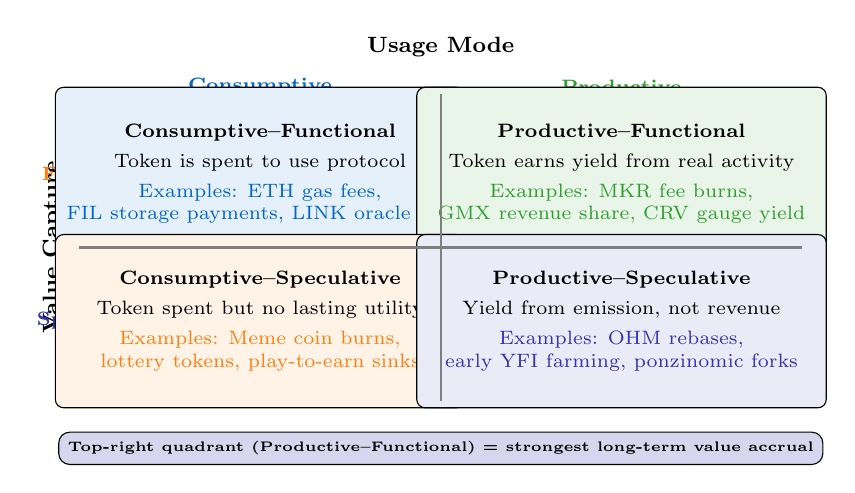
\begin{tikzpicture}[scale=0.85,
  cell/.style={draw,rounded corners=3pt,minimum width=5.2cm,minimum height=2.2cm,align=center,font=\scriptsize}]
  % Axes labels
  \node[font=\footnotesize\bfseries,rotate=90] at (-5.8,0) {Value Capture};
  \node[font=\footnotesize\bfseries] at (0,3) {Usage Mode};
  \node[font=\scriptsize,mlblue] at (-2.7,2.4) {\textbf{Consumptive}};
  \node[font=\scriptsize,mlgreen] at (2.7,2.4) {\textbf{Productive}};
  \node[font=\scriptsize,mlorange] at (-5.1,1.1) {\textbf{Functional}};
  \node[font=\scriptsize,mlpurple] at (-5.1,-1.1) {\textbf{Speculative}};
  % Quadrant cells
  \node[cell,fill=mlblue!10] at (-2.7,1.1) {
    \textbf{Consumptive--Functional}\\[1mm]
    Token is spent to use protocol\\[1mm]
    \textcolor{mlblue}{Examples: ETH gas fees,}\\
    \textcolor{mlblue}{FIL storage payments, LINK oracle fees}
  };
  \node[cell,fill=mlgreen!10] at (2.7,1.1) {
    \textbf{Productive--Functional}\\[1mm]
    Token earns yield from real activity\\[1mm]
    \textcolor{mlgreen}{Examples: MKR fee burns,}\\
    \textcolor{mlgreen}{GMX revenue share, CRV gauge yield}
  };
  \node[cell,fill=mlorange!10] at (-2.7,-1.1) {
    \textbf{Consumptive--Speculative}\\[1mm]
    Token spent but no lasting utility\\[1mm]
    \textcolor{mlorange}{Examples: Meme coin burns,}\\
    \textcolor{mlorange}{lottery tokens, play-to-earn sinks}
  };
  \node[cell,fill=mlpurple!10] at (2.7,-1.1) {
    \textbf{Productive--Speculative}\\[1mm]
    Yield from emission, not revenue\\[1mm]
    \textcolor{mlpurple}{Examples: OHM rebases,}\\
    \textcolor{mlpurple}{early YFI farming, ponzinomic forks}
  };
  % Dividing lines
  \draw[thick,mlgray] (0,-2.3) -- (0,2.3);
  \draw[thick,mlgray] (-5.4,0) -- (5.4,0);
  % Annotation
  \node[draw,fill=mllavender4,rounded corners,font=\tiny\bfseries,align=center] at (0,-3) {Top-right quadrant (Productive--Functional) = strongest long-term value accrual};
\end{tikzpicture}
}%
\end{center}
\bottomnote{Kyle Samani (Multicoin Capital): classify tokens along these axes before investing -- functional + productive = durable value}
\end{frame}

% Frame 40: Regulatory Considerations in Token Design
\begin{frame}{Regulatory Considerations in Token Design}
\begin{columns}[T]
\column{0.5\textwidth}
\begin{block}{Howey Test (SEC -- U.S.)}
\footnotesize
A token is a \textbf{security} if it satisfies ALL four prongs:
\begin{enumerate}
  \item Investment of money
  \item In a common enterprise
  \item With expectation of profits
  \item Derived from efforts of others
\end{enumerate}
\vspace{1mm}
\textbf{Implication:} Tokens with passive yield from a team's work likely qualify as securities.
\end{block}
\vspace{1mm}
\begin{exampleblock}{\footnotesize Security vs.\ Utility}
\footnotesize
\begin{itemize}
  \item \textbf{Utility:} Required to use the protocol (e.g., gas, access)
  \item \textbf{Security:} Purchased for profit expectation (e.g., revenue share)
  \item \textbf{Hybrid:} Many tokens exhibit both characteristics
\end{itemize}
\end{exampleblock}

\column{0.5\textwidth}
\begin{block}{Global Regulatory Landscape}
\footnotesize
\begin{tabular}{lp{4.2cm}}
\toprule
\textbf{Jurisdiction} & \textbf{Approach} \\
\midrule
\textbf{U.S.\ (SEC)} & Case-by-case Howey test; enforcement-driven \\
\textbf{EU (MiCA)} & Comprehensive framework; asset-referenced \& e-money tokens regulated from 2024 \\
\textbf{Singapore (MAS)} & Payment tokens exempt; security tokens under SFA \\
\textbf{Switzerland (FINMA)} & 3-tier classification: payment, utility, asset tokens \\
\textbf{UAE (VARA)} & Activity-based licensing; sandbox regime \\
\bottomrule
\end{tabular}
\end{block}
\vspace{1mm}
\begin{alertblock}{\footnotesize Design Implications}
\footnotesize
\begin{itemize}
  \item Decentralisation can move token outside Howey (``sufficiently decentralised'')
  \item Vesting, lockups, and progressive decentralisation reduce security risk
  \item Always obtain legal opinion \textbf{before} TGE
\end{itemize}
\end{alertblock}
\end{columns}
\bottomnote{Regulatory classification determines listing eligibility, investor base, and compliance costs -- get it right early}
\end{frame}

% Frame 41: Tokenomics Red Flags for Investors
\begin{frame}{Tokenomics Red Flags for Investors}
\begin{columns}[T]
\column{0.52\textwidth}
\begin{alertblock}{\footnotesize Warning Checklist}
\footnotesize
\renewcommand{\arraystretch}{1.15}
\begin{tabular}{cp{5.5cm}}
\toprule
& \textbf{Red Flag} \\
\midrule
\textcolor{mlred}{\Large$\boldsymbol{\times}$} & Insider allocation $>$ 30\% of total supply \\
\textcolor{mlred}{\Large$\boldsymbol{\times}$} & No vesting schedule for team/investor tokens \\
\textcolor{mlred}{\Large$\boldsymbol{\times}$} & Unlimited supply with no burn or sink mechanism \\
\textcolor{mlred}{\Large$\boldsymbol{\times}$} & Team tokens unlocked at TGE \\
\textcolor{mlred}{\Large$\boldsymbol{\times}$} & No clear value accrual to token holders \\
\textcolor{mlred}{\Large$\boldsymbol{\times}$} & FDV/MC ratio $>$ 10$\times$ (extreme future dilution) \\
\textcolor{mlred}{\Large$\boldsymbol{\times}$} & Yields funded by emissions, not revenue \\
\textcolor{mlred}{\Large$\boldsymbol{\times}$} & Anonymous team with no audit \\
\bottomrule
\end{tabular}
\end{alertblock}

\column{0.48\textwidth}
\begin{block}{Healthy Tokenomics Indicators}
\footnotesize
\renewcommand{\arraystretch}{1.15}
\begin{tabular}{cp{4.5cm}}
\toprule
& \textbf{Green Flag} \\
\midrule
\textcolor{mlgreen}{\Large$\checkmark$} & Community allocation $\geq$ 50\% \\
\textcolor{mlgreen}{\Large$\checkmark$} & 12--48 month vesting with cliff \\
\textcolor{mlgreen}{\Large$\checkmark$} & Real yield from protocol revenue \\
\textcolor{mlgreen}{\Large$\checkmark$} & Multiple independent audits \\
\textcolor{mlgreen}{\Large$\checkmark$} & Transparent on-chain treasury \\
\textcolor{mlgreen}{\Large$\checkmark$} & Active governance participation \\
\bottomrule
\end{tabular}
\end{block}
\vspace{2mm}
\begin{exampleblock}{\footnotesize Quick Heuristic}
\footnotesize
Score each red flag as $-1$ and each green flag as $+1$. If total score $< 0$, \textbf{investigate further} before investing. If $\leq -3$, \textbf{avoid}.
\end{exampleblock}
\end{columns}
\bottomnote{``If you can't find the sucker at the table, you're the sucker'' -- apply this to tokenomics due diligence}
\end{frame}

% Frame 42: Section 4 Summary
\begin{frame}{Section 4 Summary: Token Design Framework}
\begin{columns}[T]
\column{0.5\textwidth}
\begin{block}{7-Step Framework}
\footnotesize
\begin{enumerate}
  \item Define purpose (why does the token exist?)
  \item Choose type (utility, governance, hybrid)
  \item Design supply (fixed, inflationary, deflationary)
  \item Set distribution (fair launch, ICO, airdrop)
  \item Build incentives (staking, burns, rewards)
  \item Plan governance (voting, delegation, time-locks)
  \item Model \& simulate (agent-based testing)
\end{enumerate}
\end{block}

\column{0.5\textwidth}
\begin{block}{Solidity Patterns Covered}
\footnotesize
\begin{itemize}
  \item Linear bonding curve contract
  \item Token vesting with cliff and linear unlock
  \item Synthetix-style staking rewards
\end{itemize}
\end{block}
\vspace{2mm}
\begin{exampleblock}{\footnotesize Next Section}
\footnotesize
$\Rightarrow$ \textbf{Case Studies \& Pitfalls:} Real-world tokenomics analysis of UNI, MKR, CRV, and lessons from failures.
\end{exampleblock}
\end{columns}
\bottomnote{Theory meets practice -- the next section examines how leading protocols implement these principles}
\end{frame}

%% ============================================================
%% SECTION 5: CASE STUDIES & PITFALLS
%% ============================================================
\section{Case Studies \& Pitfalls}

\begin{frame}{}
\begin{beamercolorbox}[sep=12pt,center,rounded=true,shadow=true]{palette quaternary}
{\Large\bfseries Section 5: Case Studies \& Pitfalls}\\[6pt]
{\normalsize Real-world tokenomics successes, failures, and lessons learned}
\end{beamercolorbox}
\end{frame}

% Frame 40: UNI -- Governance Token Design
\begin{frame}{Case Study: UNI -- Governance Token Design}
\begin{columns}[T]
\column{0.5\textwidth}
\begin{block}{Token Overview}
\footnotesize
\begin{tabular}{ll}
\toprule
\textbf{Property} & \textbf{Value} \\
\midrule
Type & Governance \\
Max Supply & 1 billion UNI \\
Distribution & 60\% community, 21.5\% team \\
Launch & Sept 2020 (retroactive airdrop) \\
Value Capture & Governance only (fee switch pending) \\
\bottomrule
\end{tabular}
\end{block}
\vspace{2mm}
\begin{exampleblock}{\footnotesize Strengths}
\footnotesize
\begin{itemize}
  \item Retroactive airdrop rewarded genuine users
  \item 400 UNI to 250K+ addresses (``fair'' distribution)
  \item Strong brand and community loyalty
\end{itemize}
\end{exampleblock}

\column{0.5\textwidth}
\begin{alertblock}{\footnotesize Weaknesses}
\footnotesize
\begin{itemize}
  \item \textbf{No fee switch:} UNI holders don't earn protocol fees
  \item \textbf{Low turnout:} 3--5\% governance participation
  \item \textbf{Whale dominance:} Top 10 wallets control 40\%+ voting power
  \item \textbf{2\% annual inflation} after 4-year distribution
\end{itemize}
\end{alertblock}
\vspace{2mm}
\begin{block}{Lessons Learned}
\footnotesize
\begin{itemize}
  \item Governance-only tokens struggle with value capture
  \item Retroactive airdrops create strong initial distribution
  \item Delegation helps but doesn't solve low turnout
\end{itemize}
\end{block}
\end{columns}
\bottomnote{UNI's fee switch debate highlights the tension between protocol growth and token holder returns}
\end{frame}

% Frame 41: MKR/DAI -- Dual-Token Stability
\begin{frame}{Case Study: MKR/DAI -- Dual-Token System}
\begin{columns}[T]
\column{0.55\textwidth}
\begin{block}{Dual-Token Architecture}
\footnotesize
\begin{itemize}
  \item \textbf{DAI:} Stablecoin pegged to \$1 (user-facing)
  \item \textbf{MKR:} Governance + recapitalisation token
\end{itemize}
\end{block}
\vspace{1mm}
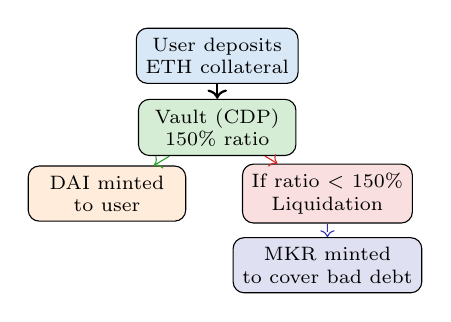
\begin{tikzpicture}[scale=0.7,
  box/.style={draw,rounded corners,minimum width=2cm,minimum height=0.7cm,font=\scriptsize,align=center}]
  \node[box,fill=mlblue!15] (user) at (0,2.5) {User deposits\\ETH collateral};
  \node[box,fill=mlgreen!20] (vault) at (0,1.2) {Vault (CDP)\\150\% ratio};
  \node[box,fill=mlorange!15] (dai) at (-2,0) {DAI minted\\to user};
  \node[box,fill=mlred!15] (liq) at (2,0) {If ratio $<$ 150\%\\Liquidation};
  \node[box,fill=mlpurple!15] (mkr) at (2,-1.3) {MKR minted\\to cover bad debt};
  \draw[->,thick] (user) -- (vault);
  \draw[->,mlgreen] (vault) -- (dai);
  \draw[->,mlred] (vault) -- (liq);
  \draw[->,mlpurple,dashed] (liq) -- (mkr);
\end{tikzpicture}

\column{0.45\textwidth}
\begin{block}{MKR Tokenomics}
\footnotesize
\begin{itemize}
  \item \textbf{Fee revenue:} Stability fees paid in DAI, used to buy and burn MKR
  \item \textbf{Backstop:} If system insolvent, new MKR is minted (dilution penalty)
  \item \textbf{Governance:} MKR holders set risk parameters
\end{itemize}
\end{block}
\vspace{2mm}
\begin{exampleblock}{\footnotesize Key Innovation}
\footnotesize
MKR holders bear the downside risk (dilution in crisis) and earn the upside (burn from fees). This aligns incentives for good governance.
\end{exampleblock}
\end{columns}
\bottomnote{MakerDAO pioneered the dual-token model -- MKR aligns governance with risk bearing}
\end{frame}

% Frame 42: CRV -- Vote-Escrowed Tokenomics
\begin{frame}{Case Study: CRV -- Vote-Escrowed Tokenomics (veCRV)}
\begin{columns}[T]
\column{0.55\textwidth}
\begin{block}{veCRV Mechanism}
\footnotesize
\begin{itemize}
  \item Lock CRV for 1 week to 4 years $\rightarrow$ receive veCRV
  \item veCRV = non-transferable, decays linearly to zero
  \item More lock time $=$ more voting power and yield boost
\end{itemize}
\end{block}
\vspace{1mm}
\begin{block}{veCRV Formula}
\footnotesize
\[
\text{veCRV} = \text{CRV} \times \frac{t_{\text{remaining}}}{t_{\max}}
\]
where $t_{\max} = 4$ years. Locking 100 CRV for 4 years gives 100 veCRV; for 1 year gives 25 veCRV.
\end{block}
\vspace{1mm}
\begin{exampleblock}{\footnotesize Benefits}
\footnotesize
\begin{itemize}
  \item Up to 2.5$\times$ yield boost for LPs
  \item Voting power over CRV emissions (gauge weights)
  \item Share of 50\% of protocol trading fees
\end{itemize}
\end{exampleblock}

\column{0.45\textwidth}
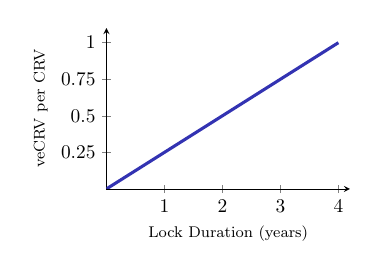
\begin{tikzpicture}[scale=0.7]
\begin{axis}[
  xlabel={\footnotesize Lock Duration (years)},
  ylabel={\footnotesize veCRV per CRV},
  width=6cm,height=4.5cm,
  axis lines=left,
  ymin=0,ymax=1.1,xmin=0,xmax=4.2,
  xtick={1,2,3,4},
  ytick={0.25,0.5,0.75,1.0}]
\addplot[mlpurple,ultra thick,domain=0:4,samples=50] {x/4};
\end{axis}
\end{tikzpicture}
\vspace{1mm}
\footnotesize
\begin{alertblock}{\footnotesize The Curve Wars}
\footnotesize
Protocols bribe veCRV holders to direct CRV emissions to their pools. Convex Finance controls 40\%+ of veCRV.
\end{alertblock}
\end{columns}
\bottomnote{veCRV solved mercenary capital -- long-term lockers govern the protocol, reducing velocity}
\end{frame}

% Frame 43: LUNA/UST -- Death Spiral Case Study
\begin{frame}{Case Study: LUNA/UST -- The \$40B Death Spiral}
\begin{columns}[T]
\column{0.55\textwidth}
\begin{block}{Algorithmic Stablecoin Mechanism}
\footnotesize
\begin{itemize}
  \item UST peg maintained by mint/burn with LUNA
  \item \$1 UST can always be redeemed for \$1 of LUNA
  \item If UST $<$ \$1: burn UST, mint LUNA (arbitrage profit)
  \item If UST $>$ \$1: burn LUNA, mint UST
\end{itemize}
\end{block}
\vspace{1mm}
\begin{alertblock}{\footnotesize What Went Wrong (May 2022)}
\footnotesize
\begin{enumerate}
  \item Large UST sell-off $\rightarrow$ UST depegged to \$0.98
  \item Arbitrageurs burned UST, minted massive LUNA
  \item LUNA supply exploded: 350M $\rightarrow$ 6.5 trillion
  \item LUNA price collapsed $\rightarrow$ UST further depegged
  \item Reflexive death spiral: both assets $\rightarrow$ \$0
\end{enumerate}
\end{alertblock}

\column{0.45\textwidth}
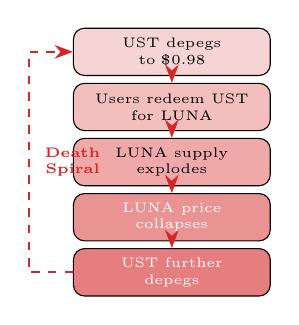
\begin{tikzpicture}[scale=0.7,
  box/.style={draw,rounded corners,minimum width=2.5cm,minimum height=0.6cm,font=\tiny,align=center}]
  \node[box,fill=mlred!20] (s1) at (0,4) {UST depegs\\to \$0.98};
  \node[box,fill=mlred!30] (s2) at (0,3) {Users redeem UST\\for LUNA};
  \node[box,fill=mlred!40] (s3) at (0,2) {LUNA supply\\explodes};
  \node[box,fill=mlred!50,text=white] (s4) at (0,1) {LUNA price\\collapses};
  \node[box,fill=mlred!60,text=white] (s5) at (0,0) {UST further\\depegs};
  \draw[-{Stealth},thick,mlred] (s1) -- (s2);
  \draw[-{Stealth},thick,mlred] (s2) -- (s3);
  \draw[-{Stealth},thick,mlred] (s3) -- (s4);
  \draw[-{Stealth},thick,mlred] (s4) -- (s5);
  \draw[-{Stealth},thick,mlred,dashed] (s5.west) -- ++(-0.8,0) |- (s1.west);
  \node[font=\tiny\bfseries,mlred,align=center] at (-1.8,2) {Death\\Spiral};
\end{tikzpicture}
\end{columns}
\bottomnote{LUNA/UST is the most expensive tokenomics failure in history -- \$40B in value destroyed in 72 hours}
\end{frame}

% Frame 44: Comparing Token Models
\begin{frame}{Comparing Real-World Token Models}
\footnotesize
\begin{tabular}{lccccc}
\toprule
\textbf{Dimension} & \textbf{UNI} & \textbf{MKR} & \textbf{CRV} & \textbf{LUNA} & \textbf{ETH} \\
\midrule
Type & Governance & Gov + Backstop & Gov + Yield & Collateral & Native coin \\
Supply & 1B fixed & Elastic & 3.03B max & Elastic & No cap \\
Value capture & Weak & Strong & Strong & Reflexive & Fee burn \\
Velocity sink & Delegation & Burn & veLock & Stake & Stake \\
Distribution & Airdrop & Sale & Mining & Sale & Mining \\
Governance & Direct vote & Direct vote & Gauge vote & Validators & -- \\
Resilience & High & High & High & \textcolor{mlred}{Failed} & High \\
\bottomrule
\end{tabular}
\vspace{3mm}
\begin{columns}[T]
\column{0.5\textwidth}
\begin{exampleblock}{\footnotesize Success Patterns}
\footnotesize
\begin{itemize}
  \item Multiple value capture mechanisms
  \item Aligned incentives (skin in the game)
  \item Velocity sinks (staking, locking)
  \item Gradual token unlock
\end{itemize}
\end{exampleblock}

\column{0.5\textwidth}
\begin{alertblock}{\footnotesize Failure Patterns}
\footnotesize
\begin{itemize}
  \item Reflexive/circular value backing
  \item Unsustainable yield promises
  \item Concentrated token holdings
  \item No intrinsic demand driver
\end{itemize}
\end{alertblock}
\end{columns}
\bottomnote{Study both successes and failures -- the difference often lies in the robustness of value capture}
\end{frame}

% Frame 45: Common Tokenomics Pitfalls
\begin{frame}{Common Tokenomics Pitfalls}
\begin{columns}[T]
\column{0.5\textwidth}
\begin{alertblock}{\footnotesize 1. Ponzi Dynamics}
\footnotesize
\begin{itemize}
  \item Returns funded by new entrants, not real yield
  \item Steep bonding curves that only reward early buyers
  \item \textbf{Red flag:} ``guaranteed'' yields $>$ 100\% APY
\end{itemize}
\end{alertblock}
\vspace{1mm}
\begin{alertblock}{\footnotesize 2. Governance Capture}
\footnotesize
\begin{itemize}
  \item Whales accumulate voting power
  \item Pass proposals benefiting insiders
  \item \textbf{Red flag:} Top 10 addresses hold $>$50\% supply
\end{itemize}
\end{alertblock}
\vspace{1mm}
\begin{alertblock}{\footnotesize 3. Emission Cliff}
\footnotesize
\begin{itemize}
  \item High initial rewards attract users
  \item Rewards drop sharply $\rightarrow$ users leave
  \item TVL collapses, token price follows
\end{itemize}
\end{alertblock}

\column{0.5\textwidth}
\begin{alertblock}{\footnotesize 4. Insufficient Liquidity}
\footnotesize
\begin{itemize}
  \item Thin order books cause extreme volatility
  \item Large holders cannot exit without crashing price
  \item \textbf{Solution:} Ensure deep initial liquidity
\end{itemize}
\end{alertblock}
\vspace{1mm}
\begin{alertblock}{\footnotesize 5. Regulatory Risk}
\footnotesize
\begin{itemize}
  \item Token classified as unregistered security
  \item SEC enforcement actions (XRP, LBRY)
  \item \textbf{Mitigation:} Legal opinion before launch
\end{itemize}
\end{alertblock}
\vspace{1mm}
\begin{exampleblock}{\footnotesize Due Diligence Questions}
\footnotesize
\begin{itemize}
  \item Where do the yields come from?
  \item Who bears the risk?
  \item What happens if price drops 80\%?
  \item Is the token actually needed?
\end{itemize}
\end{exampleblock}
\end{columns}
\bottomnote{``If you can't explain where the yield comes from, you are the yield'' -- crypto investing wisdom}
\end{frame}

% Frame 46: Tokenomics Analysis Framework
\begin{frame}{Tokenomics Analysis Framework}
\begin{center}
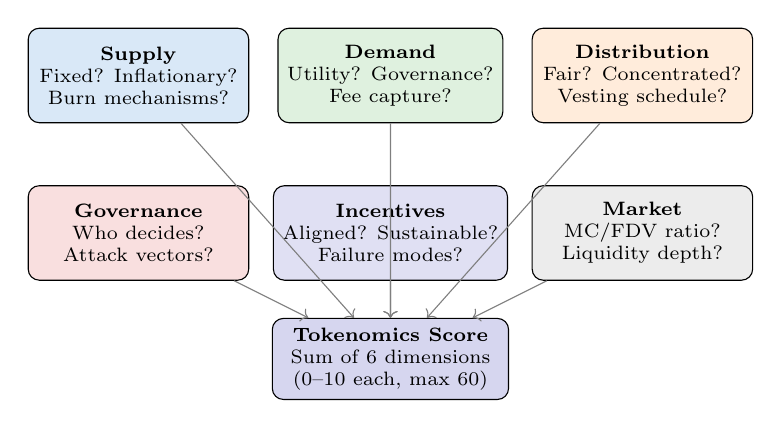
\begin{tikzpicture}[scale=0.8,
  dim/.style={draw,rounded corners=4pt,minimum width=2.8cm,minimum height=1.2cm,align=center,font=\scriptsize}]
  \node[dim,fill=mlblue!15] (supply) at (0,2) {\textbf{Supply}\\Fixed? Inflationary?\\Burn mechanisms?};
  \node[dim,fill=mlgreen!15] (demand) at (4,2) {\textbf{Demand}\\Utility? Governance?\\Fee capture?};
  \node[dim,fill=mlorange!15] (dist) at (8,2) {\textbf{Distribution}\\Fair? Concentrated?\\Vesting schedule?};
  \node[dim,fill=mlred!15] (gov) at (0,-0.5) {\textbf{Governance}\\Who decides?\\Attack vectors?};
  \node[dim,fill=mlpurple!15] (incent) at (4,-0.5) {\textbf{Incentives}\\Aligned? Sustainable?\\Failure modes?};
  \node[dim,fill=mlgray!15] (market) at (8,-0.5) {\textbf{Market}\\MC/FDV ratio?\\Liquidity depth?};
  % Score box
  \node[draw,fill=mllavender4,rounded corners,minimum width=3cm,font=\scriptsize,align=center] (score) at (4,-2.5) {\textbf{Tokenomics Score}\\Sum of 6 dimensions\\(0--10 each, max 60)};
  \draw[->,mlgray] (supply) -- (score);
  \draw[->,mlgray] (demand) -- (score);
  \draw[->,mlgray] (dist) -- (score);
  \draw[->,mlgray] (gov) -- (score);
  \draw[->,mlgray] (incent) -- (score);
  \draw[->,mlgray] (market) -- (score);
\end{tikzpicture}
\end{center}
\bottomnote{Use this 6-dimension framework to systematically evaluate any token's economic design}
\end{frame}

% Frame 47: Future of Tokenomics
\begin{frame}{The Future of Tokenomics}
\begin{columns}[T]
\column{0.5\textwidth}
\begin{block}{Emerging Trends}
\footnotesize
\begin{enumerate}
  \item \textbf{Real-World Assets (RWA):} Tokenised treasuries, real estate, commodities
  \item \textbf{Account abstraction:} Gas-free token interactions (ERC-4337)
  \item \textbf{Soulbound tokens (SBTs):} Non-transferable identity/reputation
  \item \textbf{Dynamic NFTs:} Token properties that evolve based on on-chain data
  \item \textbf{Restaking:} EigenLayer-style shared security tokenomics
\end{enumerate}
\end{block}

\column{0.5\textwidth}
\begin{block}{Regulatory Evolution}
\footnotesize
\begin{itemize}
  \item EU MiCA framework (effective 2024)
  \item SEC vs.\ Ripple precedent
  \item ``Sufficiently decentralised'' doctrine
  \item Compliance-by-design tokenomics
\end{itemize}
\end{block}
\vspace{2mm}
\begin{exampleblock}{\footnotesize Research Frontiers}
\footnotesize
\begin{itemize}
  \item Agent-based token simulation (cadCAD, TokenSPICE)
  \item Formal verification of token mechanisms
  \item Cross-chain tokenomics and bridge design
  \item AI-assisted mechanism design
\end{itemize}
\end{exampleblock}
\end{columns}
\bottomnote{Tokenomics is a young field -- the best designs of the next decade haven't been invented yet}
\end{frame}

% Frame 48: Course Summary & Key Takeaways
\begin{frame}{Lecture Summary \& Key Takeaways}
\begin{columns}[T]
\column{0.5\textwidth}
\begin{block}{5 Sections Covered}
\footnotesize
\begin{enumerate}
  \item \textbf{Token Fundamentals:} Types, supply models, velocity
  \item \textbf{Bonding Curves:} Linear, polynomial, Bancor, sigmoid, $xy=k$
  \item \textbf{Incentive Design:} Game theory, staking, slashing, MEV
  \item \textbf{Design Framework:} 7-step methodology, vesting, launch
  \item \textbf{Case Studies:} UNI, MKR, CRV, LUNA failures
\end{enumerate}
\end{block}
\vspace{2mm}
\begin{exampleblock}{\footnotesize Solidity Patterns}
\footnotesize
\begin{itemize}
  \item Linear bonding curve (mint/burn)
  \item Token vesting with cliff
  \item Synthetix-style staking rewards
\end{itemize}
\end{exampleblock}

\column{0.5\textwidth}
\begin{block}{Golden Rules of Tokenomics}
\footnotesize
\begin{enumerate}
  \item Design for rational, self-interested actors
  \item Create sinks to reduce velocity
  \item Align incentives: skin in the game
  \item Never back a token with itself (no reflexivity)
  \item Simulate before deploying
  \item Start with ``Does this need a token?''
\end{enumerate}
\end{block}
\vspace{2mm}
\begin{block}{Further Reading}
\footnotesize
\begin{itemize}
  \item Vitalik Buterin: ``Token Sales'' (2017)
  \item Placeholder VC: ``Cryptonetwork Governance''
  \item Gauntlet: cadCAD simulation framework
\end{itemize}
\end{block}
\end{columns}
\bottomnote{The best tokenomics creates systems where selfish behaviour produces collective benefit}
\end{frame}

% Frame 49: Questions & Discussion
\begin{frame}{Questions \& Discussion}
\begin{center}
\vspace{5mm}
{\Large\textbf{Thank you!}}\\[8mm]
{\large Questions \& Discussion}\\[8mm]
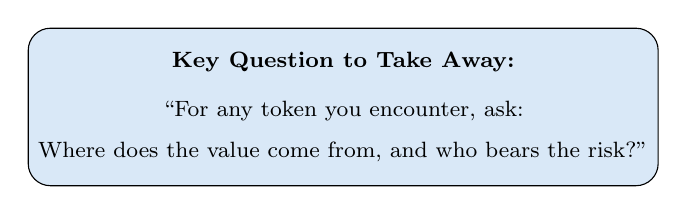
\begin{tikzpicture}[scale=0.8]
  \node[draw,fill=mlblue!15,rounded corners=8pt,minimum width=8cm,minimum height=2cm,align=center] {
    \footnotesize\textbf{Key Question to Take Away:}\\[2mm]
    \footnotesize ``For any token you encounter, ask:\\[1mm]
    \footnotesize Where does the value come from, and who bears the risk?''
  };
\end{tikzpicture}
\end{center}
\bottomnote{Contact: joerg.osterrieder@{university email} | Course materials available on GitHub Pages}
\end{frame}

\end{document}
